\exercisesection{5}

\begin{enumerate}
\def\labelenumi{\arabic{enumi}.}
\tightlist
\item
  Let A be a commutative ring and \(\mathfrak{I}\) an ideal of A. An A-module M is called absolutely Hausdorff with respect to \(\mathfrak{I}\) if, for every finitely generated A-module N, the A-module N \(\otimes_{\mathrm{A}}\) M is Hausdorff with the \(\mathfrak{I}\) -adic topology; an absolutely Hausdorff A-module is ideally Hausdorff.
\end{enumerate}

\begin{enumerate}
\def\labelenumi{(\alph{enumi})}
\item
  For M to be absolutely Hausdorff with respect to \(\mathfrak{I}\) , it is necessary and sufficient that, for every finitely generated A-module N and every submodule \(\mathbf{N}'\) of N, \(\operatorname{Im}(\mathbf{N}' \otimes_{\mathbf{A}} \mathbf{M})\) be closed in \(\mathbf{N} \otimes_{\mathbf{A}} \mathbf{M}\) with the \(\mathfrak{I}\) -adic topology.
\item
  Let B be a commutative A-algebra and \(\mathfrak{L}\) an ideal of B containing \(\mathfrak{I}B\) . If M is an absolutely Hausdorff B-module with respect to \(\mathfrak{L}\) , M is an absolutely Hausdorff A-module with respect to \(\mathfrak{I}\) .
\end{enumerate}

\begin{enumerate}
\def\labelenumi{\arabic{enumi}.}
\setcounter{enumi}{1}
\item
  Show that every Z-module which is Hausdorff with the p-adic topology (p a prime number) is ideally Hausdorff, but give an example of a finitely generated Z-module which is Hausdorff but not absolutely Hausdorff with respect to p (use Exercise 1 (a)).
\item
  With the notation of Exercise 11 of §3, let N be the submodule of \(\hat{\mathbf{E}}\) which is the closure in \(\hat{\mathbf{E}}\) of the submodule of \(\hat{\mathbf{E}}\) generated by the vectors \(pe_{2n-1} - p^n e_{2n} (n \geqslant 1)\) and let M = \(\hat{\mathbf{E}}/\mathbf{N}\) . Show that under the \(p\) -adic topology the submodule \(p\mathbf{M}\) of M is not closed in M and deduce that M is a \(\mathbf{Z}_p\) -module which is ideally Hausdorff but not absolutely Hausdorff with respect to \(p\) .
\end{enumerate}

¶ 4. Let A be a commutative ring, \(\mathfrak{I}\) an ideal of A and S = 1 + \(\mathfrak{I}\). Show that, if M is an absolutely Hausdorff A-module with respect to \(\mathfrak{I}\), then S \(^{-1}\) M = M, in other words, for all \(a \in\) S, \(x \mapsto ax\) is a bijection of M onto itself. (Show first that the hypothesis that M is Hausdorff with the \(\mathfrak{I}\)-adic topology implies that \(x \mapsto ax\) is injective; then prove that the submodule aM of M is dense in M with the \(\mathfrak{I}\)-adic topology and use Exercise 1 (a).)

\begin{enumerate}
\def\labelenumi{\arabic{enumi}.}
\setcounter{enumi}{4}
\tightlist
\item
  Take \(\mathbf{A} = \mathbf{Z}\) and \(\mathfrak{I} = p\mathbf{Z}\) , where \(p\) is prime.
\end{enumerate}

\begin{enumerate}
\def\labelenumi{(\alph{enumi})}
\item
  Show that, if \(q\) is a prime number distinct from \(p\) , the \(\mathbf{Z}\) -module \(\mathbf{Z} / q\mathbf{Z}\) satisfies property (ii) of Theorem 1, but not property (i).
\item
  Show that the \(\mathbf{Z}\) -module \(\mathbf{Q} / \mathbf{Z}\) satisfies property (iv) of Theorem 1 but not property (ii).
\end{enumerate}

\begin{enumerate}
\def\labelenumi{\arabic{enumi}.}
\setcounter{enumi}{5}
\tightlist
\item
  Let A be a commutative Noetherian ring, \(\mathfrak{I}\) an ideal of A and M an A-module. Show that condition (v) of Theorem 1 is equivalent to the following:
\end{enumerate}

(v') For every finitely generated A-module N and every submodule N' of N, the canonical mapping \((\mathbf{M} \otimes_{\mathbf{A}} \mathbf{N}')^{\wedge} \to (\mathbf{M} \otimes_{\mathbf{A}} \mathbf{N})^{\wedge}\) (where the two sides are the Hausdorff completions with respect to the \(\mathfrak{I}\) -adic topologies on M \(\otimes_{A} N'\) and M \(\otimes_{A} N\) respectively) is injective. (To prove that (v) implies (v'), argue as in part (E) of the proof of Theorem 1. To see that (v') implies (v), consider A-modules N annihilated by a power of \(\mathfrak{I}\).)

¶ 7. Let \((A_{\lambda}, f_{\mu\lambda})\) be a directed direct system of Noetherian local rings; if \(m_{\lambda}\) is the maximal ideal of \(A_{\lambda}\) , suppose that, for \(\lambda \leqslant \mu\) , \(m_{\mu} = m_{\lambda}A_{\mu}\) and that \(A_{\mu}\) is a flat \(A_{\lambda}\) -module. Show then that \(A = \lim A_{\lambda}\) is Noetherian and a flat \(A_{\lambda}\) -module for all \(\lambda\) . (If \(m = m_{\lambda}A\) is the maximal ideal of \(A\) (Chapter II, § 3, Exercise 16), show that on \(A\) the m-adic topology is Hausdorff, observing that \(A\) is a faithfully flat \(A_{\lambda}\) -module for all \(\lambda\) . Then prove that, if \(\hat{A}\) is the completion of \(A\) with respect to the m-adic topology, \(\hat{A}\) is Noetherian, using § 2, no. 10, Corollary 5 to Theorem 2; finally, prove that, for all \(\lambda\) , \(\hat{A}\) is a flat \(A_{\lambda}\) -module using Theorem 1 of no. 2 and Proposition 2 of no. 3.)

¶ 8. Let A be a Noetherian local ring, m its maximal ideal and k = A/m its residue field. Let K be an extension of k; show that there exists a local homomorphism from A to a Noetherian local ring B such that B/mB is isomorphic to K and B is a flat A-module. (Consider first the case where \(\mathbf{K} = k(t)\) , distinguishing two cases according to whether t is algebraic or transcendental over k; consider next a family \((\mathrm{K}_{\lambda})\) of subfields of K containing k, which is well ordered by inclusion and such that, if \(K_{\lambda}\) has a predecessor \(\mathrm{K}_{\mu}, \mathrm{K}_{\lambda} = \mathrm{K}_{\mu}(t_{\mu})\) for some \(t_{\mu} \in K_{\mu}\) . Finally, apply Exercise 7.)

CHAPTER IV(*)

\chapter{Associated Prime Ideals and Primary Decomposition}

(*) The results of this chapter depend only on Books I to VI and Chapters I to III of this Book, excluding Chapter I, § 4 and Chapter III, § 5.

All the rings considered in this chapter are assumed to be commutative and to possess a unit element; all the ring homomorphisms are assumed to map unit element to unit element. By a subring of a ring A we shall mean a subring containing the unit element of A.

Recall that for every A-module E and all \(x \in E\) , \(\text{Ann}(x)\) denotes the annihilator of x, the set of \(a \in A\) such that ax = 0.

\section{PRIME IDEALS ASSOCIATED WITH A MODULE}

\subsection{Definition of associated prime ideals}

DEFINITION 1. Let M be a module over a ring A. A prime ideal p is said to be associated with M if there exists \(x \in M\) such that p is equal to the annihilator of x. The set of prime ideals associated with M is denoted by \(\operatorname{Ass}_{\mathbf{A}}(\mathbf{M})\) , or simply \(\operatorname{Ass}(\mathbf{M})\) .

* Example. Let \(a\) be an ideal in the polynomial ring \(A = \mathbf{C}[X_1, \ldots, X_r]\) , \(V\) the corresponding affine algebraic variety and \(V_1, \ldots, V_p\) the irreducible components of \(V\) . If \(M\) is taken to be the ring \(A/a\) of functions which are regular on \(V\) , the set of prime ideals associated with \(M\) consists of the ideals of \(V_1, \ldots, V_p\) and in general other prime ideals each of which contains one of the ideals of the \(V_1\) .

As the annihilator of 0 is A, an element \(x \in \mathbf{M}\) whose annihilator is a prime ideal is necessarily \(\neq 0\) . To say that a prime ideal \(p\) is associated with M amounts to saying that M contains a submodule isomorphic to A/p (namely Ax, for all \(x \in M\) whose annihilator is p).

If an A-module M is the union of a family \((M_{t})_{t\in I}\) of submodules, then clearly

\[
\operatorname{Ass} (\mathbf {M}) = \bigcup_ {\iota \in I} \operatorname{Ass} \left(\mathbf {M} _ {\iota}\right).\tag{1}
\]

PROPOSITION 1. For every prime ideal \(\mathfrak{p}\) of a ring \(\mathbf{A}\) and every submodule \(\mathbf{M} \neq 0\) of \(\mathbf{A} / \mathfrak{p}\) , \(\operatorname{Ass}(\mathbf{M}) = \{\mathfrak{p}\}\) .

As the ring A/p is an integral domain, the annihilator of an element \(\neq0\) of A/p is p.

PROPOSITION 2. Let M be a module over a ring A. Every maximal element of the set of ideals Ann(x) of A, where x runs through the set of elements \(\neq0\) of M, belongs to Ass(M).

Let \(\mathfrak{a} = \operatorname{Ann}(x)\) ( \(x \in \mathbf{M}, x \neq 0\) ) be such a maximal element; it is sufficient to show that \(\mathfrak{a}\) is prime. As \(x \neq 0\) , \(\mathfrak{a} \neq \mathbf{A}\) . Let \(b, c\) be elements of \(\mathbf{A}\) such that \(bc \in \mathfrak{a}\) and \(c \notin \mathfrak{a}\) . Then \(cx \neq 0\) , \(b \in \operatorname{Ann}(cx)\) and \(\mathfrak{a} \subset \operatorname{Ann}(cx)\) . As \(\mathfrak{a}\) is maximal, \(\operatorname{Ann}(cx) = \mathfrak{a}\) , whence \(b \in \mathfrak{a}\) , so that \(\mathfrak{a}\) is prime.

COROLLARY 1. Let M be a module over a Noetherian ring A. Then the condition \(M \neq \{0\}\) is equivalent to \(\operatorname{Ass}(M) \neq \varnothing\) .

If \(M = \{0\}\) , clearly \(\text{Ass}(M)\) is empty (without any hypothesis on A). If \(M \neq \{0\}\) , the set of ideals of the form \(\text{Ann}(x)\) , where \(x \in M\) and \(x \neq 0\) , is non-empty and consists of ideals \(\neq A\) ; as A is Noetherian, this set has a maximal element; then it suffices to apply Proposition 2.

COROLLARY 2. Let A be a Noetherian ring, M an A-module and a an element of A. For the homothety on M with ratio a to be injective, it is necessary and sufficient that a belong to no prime ideal associated with M.

If \(a\) belongs to a prime ideal \(\mathfrak{p} \in \operatorname{Ass}(\mathbf{M})\) , then \(\mathfrak{p} = \operatorname{Ann}(x)\) , where \(x \in \mathbf{M}\) , \(x \neq 0\) ; whence \(ax = 0\) and the homothety with ratio \(a\) is not injective. Conversely, if \(ax = 0\) for some \(x \in \mathbf{M}\) such that \(x \neq 0\) , then \(Ax \neq \{0\}\) , whence \(\operatorname{Ass}(x) \neq \varnothing\) (Corollary 1). Let \(\mathfrak{p} \in \operatorname{Ass}(\mathbf{A}x)\) ; then obviously \(\mathfrak{p} \in \operatorname{Ass}(\mathbf{M})\) and \(\mathfrak{p} = \operatorname{Ann}(bx)\) , where \(b \in \mathbf{A}\) ; whence \(a \in \mathfrak{p}\) , since \(abx = 0\) .

COROLLARY 3. The set of divisors of zero in a Noetherian ring A is the union of the ideals \(\mathfrak{p} \in \operatorname{Ass}(A)\) .

PROPOSITION 3. Let A be a ring, M an A-module and N a submodule of N. Then

\[
\operatorname{Ass} (\mathbf {N}) \subset \operatorname{Ass} (\mathbf {M}) \subset \operatorname{Ass} (\mathbf {N}) \cup \operatorname{Ass} (\mathbf {M} / \mathbf {N}).\tag{2}
\]

The inclusion \(\operatorname{Ass}(\mathbf{N}) \subset \operatorname{Ass}(\mathbf{M})\) is obvious. Let \(\mathfrak{p} \in \operatorname{Ass}(\mathbf{M})\) , \(\mathbf{E}\) be a submodule of \(\mathbf{M}\) isomorphic to \(\mathbf{A} / \mathfrak{p}\) and \(\mathbf{F} = \mathbf{E} \cap \mathbf{N}\) . If \(\mathbf{F} = \{0\}\) , \(\mathbf{E}\) is isomorphic to a submodule of M/N, whence \(\mathfrak{p} \in \operatorname{Ass}(M/N)\) . If \(F \neq \{0\}\) , the annihilator of every element \(\neq 0\) of F is p (Proposition 1) and hence \(\mathfrak{p} \in \operatorname{Ass}(F) \subset \operatorname{Ass}(N)\) .

COROLLARY 1. If an A-module M is the direct sum of a family \((\mathbf{M}_t)_{t \in I}\) of submodules, then \(\operatorname{Ass}(\mathbf{M}) = \bigcup_{t \in I} \operatorname{Ass}(\mathbf{M}_t)\) .

It may be reduced to the case where I is finite by means of (1), then to the case where \(\operatorname{Card}(I) = 2\) by induction on \(\operatorname{Card}(I)\) . Then let \(I = \{i, j\}\) , where \(i \neq j\) ; as \(M/M_{i}\) is isomorphic to \(M_{j}\) , \(\operatorname{Ass}(M) \subset \operatorname{Ass}(M_{i}) \cup \operatorname{Ass}(M_{j})\) (Proposition 3); moreover, \(\operatorname{Ass}(M_{i})\) and \(\operatorname{Ass}(M_{j})\) are contained in \(\operatorname{Ass}(M)\) (Proposition 3), whence the result.

COROLLARY 2. Let M be an A-module and \((\mathbf{Q}_i)_{i\in I}\) a finite family of submodules of M. If \(\bigcap_{i\in I} \mathbf{Q}_i = \{0\}\) , then

\[
\operatorname{Ass} (\mathbf {M}) \subset \bigcup_ {i \in I} \operatorname{Ass} (\mathbf {M} / \mathbf {Q} _ {i}).
\]

The canonical mapping \(\mathbf{M} \to \bigoplus_{i \in I} (\mathbf{M} / \mathbf{Q}_i)\) is injective; then it suffices to apply Proposition 3 and its Corollary 1.

PROPOSITION 4. Let M be an A-module and \(\Phi\) a subset of \(\operatorname{Ass}(\mathbf{M})\) . Then there exists a submodule N of M such that \(\operatorname{Ass}(\mathbf{N}) = \operatorname{Ass}(\mathbf{M}) - \Phi\) and \(\operatorname{Ass}(\mathbf{M}/\mathbf{N}) = \Phi\) .

Let \(\mathfrak{E}\) be the set of submodules \(P\) of \(M\) such that \(\operatorname{Ass}(P) \subset \operatorname{Ass}(M) - \Phi\) . Formula (1) shows that the set \(\mathfrak{E}\) , ordered by inclusion, is inductive; moreover, \(\{0\} \in \mathfrak{E}\) and hence \(\mathfrak{E} \neq \varnothing\) . Let \(N\) be a maximal element of \(\mathfrak{E}\) . Then \(\operatorname{Ass}(N) \subset \operatorname{Ass}(M) - \Phi\) . We shall see that \(\operatorname{Ass}(M/N) \subset \Phi\) , which, by Proposition 3, will complete the proof. Let \(p \in \operatorname{Ass}(M/N)\) ; then \(M/N\) contains a submodule \(F/N\) isomorphic to \(A/p\) . By Propositions 1 and 3, \(\operatorname{Ass}(F) \subset \operatorname{Ass}(N) \cup \{p\}\) . Since \(N\) is maximal in \(\mathfrak{E}\) , \(F \notin \mathfrak{E}\) and hence \(p \in \Phi\) .

\subsection{Localization of associated prime ideals}

PROPOSITION 5. Let A be a ring, S a multiplicative subset of A, \(\Phi\) the set of prime ideals of A which do not meet S and M an A-module. Then:

\begin{enumerate}
\def\labelenumi{(\roman{enumi})}
\item
  The mapping \(\mathfrak{p} \mapsto \mathrm{S}^{-1}\mathfrak{p}\) is a bijection of \(\operatorname{Ass}_{\mathbf{A}}(\mathbf{M}) \cap \Phi\) onto a subset of \(\operatorname{Ass}_{\mathbf{S}^{-1}\mathbf{A}}(\mathbf{S}^{-1}\mathbf{M})\) .
\item
  If \(\mathfrak{p} \in \Phi\) is a finitely generated ideal and \(S^{-1}\mathfrak{p} \in \operatorname{Ass}_{\mathbf{S}^{-1}\mathbf{A}}(\mathbf{S}^{-1}\mathbf{M})\) , then \(\mathfrak{p} \in \operatorname{Ass}_A(M)\) .
\end{enumerate}

Recall (Chapter II, § 2, no. 5, Proposition 11) that the mapping \(\mathfrak{p} \mapsto \mathrm{S}^{-1}\mathfrak{p}\) is a bijection of \(\Phi\) onto the set of prime ideals of \(\mathrm{S}^{-1}\mathrm{A}\) . If \(\mathfrak{p} \in \operatorname{Ass}_{\mathbf{A}}(\mathbf{M}) \cap \Phi\) , \(\mathfrak{p}\) is the annihilator of a monogenous submodule \(\mathbf{N}\) of \(\mathbf{M}\) ; then \(\mathrm{S}^{-1}\mathfrak{p}\) is the annihilator of the monogenous submodule \(\mathrm{S}^{-1}\mathrm{N}\) of \(\mathrm{S}^{-1}\mathrm{M}\) (Chapter II, § 2, no. 4, formula (9)) and hence \(\mathbf{S}^{-1}\mathfrak{p}\in\mathrm{Ass}_{\mathbf{S}^{-1}\mathbf{A}}(\mathbf{S}^{-1}\mathbf{M})\) . Conversely, suppose that \(\mathfrak{p}\in\Phi\) is finitely generated and such that \(\mathbf{S}^{-1}\mathfrak{p}\) is associated with \(\mathbf{S}^{-1}\mathbf{M}\) ; then there exists \(x\in\mathbf{M}\) and \(t\in\mathbf{S}\) such that \(\mathbf{S}^{-1}\mathfrak{p}\) is the annihilator of \(x/t\) . Let \((a_{i})_{1\leqslant i\leqslant n}\) be a system of generators of \(\mathfrak{p}\) ; then \((a_{i}/1)(x/t)=0\) and hence there exists \(s_{i}\in\mathbf{S}\) such that \(s_{i}a_{i}x=0\) ( \(1\leqslant i\leqslant n\) ). Let us write \(s=s_{1}s_{2}\ldots s_{n}\) ; for all \(a\in\mathfrak{p}\) , \(sax=0\) , whence \(\mathfrak{p}\subset\mathrm{Ann}(sx)\) ; on the other hand, if \(b\in\mathbf{A}\) satisfies \(bsx=0\) , then \(b/1\in\mathbf{S}^{-1}\mathfrak{p}\) by definition, whence \(b\in\mathfrak{p}\) . Then \(\mathfrak{p}=\mathrm{Ann}(sx)\) and \(\mathfrak{p}\in\mathrm{Ass}_{\mathbf{A}}(\mathbf{M})\) .

COROLLARY. If the ring A is Noetherian, the mapping \(\mathfrak{p} \mapsto \mathrm{S}^{-1}\mathfrak{p}\) is a bijection of \(\operatorname{Ass}_{\mathbf{A}}(\mathbf{M}) \cap \Phi\) onto \(\operatorname{Ass}_{\mathbf{S}^{-1}\mathbf{A}}(\mathbf{S}^{-1}\mathbf{M})\) .

If A is not Noetherian, the mapping \(p \mapsto S^{-1}p\) of \(\operatorname{Ass}_{\mathbf{A}}(\mathbf{M}) \cap \Phi\) to \(\operatorname{Ass}_{\mathbf{S}^{-1}\mathbf{A}}(\mathbf{S}^{-1}\mathbf{M})\) is not necessarily surjective (Exercise 1).

PROPOSITION 6. Let A be a Noetherian ring, M an A-module, S a multiplicative subset of A and \(\Psi\) the set of elements of \(\operatorname{Ass}_{\mathbf{A}}(\mathbf{M})\) which do not meet S. Then the kernel N of the canonical mapping \(M \to S^{-1}M\) is the unique submodule of M which satisfies the relations

\[
\operatorname{Ass} (N) = \operatorname{Ass} (M) - \Psi , \quad \operatorname{Ass} (M / N) = \Psi .\tag{3}
\]

By Proposition 4 of no. 1, there exists a submodule \(\mathbf{N}'\) of \(\mathbf{M}\) which satisfies the relations \(\operatorname{Ass}(\mathbf{N}') = \operatorname{Ass}(\mathbf{M}) - \Psi'\) and \(\operatorname{Ass}(\mathbf{M}/\mathbf{N}') = \Psi'\) . We need to prove \(\mathbf{N}' = \mathbf{N}\) . Consider the commutative diagram

\[
\begin{array}{c} \mathrm{M} \xrightarrow {p} \mathrm{M} / \mathrm{N} ^ {\prime} \\ u \Biggl \downarrow \\ \mathrm{S} ^ {- 1} \mathrm{M} \xrightarrow [ \mathrm{S} ^ {- 1 p} ]{} \mathrm{S} ^ {- 1} (\mathrm{M} / \mathrm{N} ^ {\prime}) \end{array}
\]

where \(p, u, v\) are the canonical homomorphisms. We shall show that \(S^{-1}p\) and \(v\) are injective, which will prove that \(u\) and \(p\) have the same kernel and hence \(N' = N\) .

As \(\operatorname{Ass}(\mathbf{N}') \cap \Psi' = \varnothing\) , every element of \(\operatorname{Ass}(\mathbf{N}')\) meets S. Then \(\operatorname{Ass}_{\mathbf{S}^{-1}\mathbf{A}}(\mathbf{S}^{-1}\mathbf{N}') = \varnothing\) (Corollary to Proposition 5), whence \(\mathbf{S}^{-1}\mathbf{N}' = \{0\}\) (no. 1, Corollary 1 to Proposition 2), which proves that \(\mathbf{S}^{-1}\mathfrak{p}\) is injective (Chapter II, § 2, no. 4, Theorem 1). On the other hand, if \(x\) belongs to the kernel K of \(v\) , then \(\operatorname{Ann}(x) \cap \mathbf{S} \neq \varnothing\) (Chapter II, § 2, no. 2, Proposition 4); hence \(\operatorname{Ass}(\mathbf{K}) = \varnothing\) since \(\operatorname{Ass}(\mathbf{K}) \subset \operatorname{Ass}(\mathbf{M}/\mathbf{N}') = \Psi'\) ; we deduce that \(\mathbf{K} = \{0\}\) (no. 1, Corollary 1 to Proposition 2) and \(v\) is injective.

\subsection{Relations with the support}

Let M be a module over a ring A. Recall that the set of prime ideals p of A such that \(M_{p} \neq 0\) is called the support of M and is denoted by Supp(M) (Chapter II, §4, no. 4, Definition 5).

PROPOSITION 7. Let A be a ring and M an A-module.

\begin{enumerate}
\def\labelenumi{(\roman{enumi})}
\item
  Every prime ideal \(\mathfrak{p}\) of A containing an element of \(\operatorname{Ass}(\mathbf{M})\) belongs to \(\operatorname{Supp}(\mathbf{M})\) .
\item
  Conversely, if A is Noetherian, every ideal \(\mathfrak{p} \in \operatorname{Supp}(\mathbf{M})\) contains an element of \(\operatorname{Ass}(\mathbf{M})\) .
\end{enumerate}

If \(\mathfrak{p}\) contains an element \(\mathfrak{q}\) of \(\operatorname{Ass}(\mathbf{M})\) , then \(\mathfrak{q} \cap (\mathbf{A} - \mathfrak{p}) = \varnothing\) and hence, if we write \(\mathbf{S} = \mathbf{A} - \mathfrak{p}\) , \(\mathbf{S}^{-1}\mathfrak{p}\) is a prime ideal associated with \(\mathbf{S}^{-1}\mathbf{M} = \mathbf{M}_{\mathfrak{p}}\) (no. 2, Proposition 5) and a fortiori \(\mathbf{M}_{\mathfrak{p}} \neq 0\) , hence \(\mathfrak{p} \in \operatorname{Supp}(\mathbf{M})\) . Conversely, if \(\mathbf{A}\) is Noetherian, so is \(\mathbf{A}_{\mathfrak{p}}\) (Chapter II, § 2, no. 4, Corollary 2 to Proposition 10). If \(\mathbf{M}_{\mathfrak{p}} \neq 0\) , then \(\operatorname{Ass}_{\mathbf{A}_{\mathfrak{p}}}(\mathbf{M}_{\mathfrak{p}}) \neq 0\) (no. 1, Corollary 1 to Proposition 2) and hence there exists \(\mathfrak{q} \in \operatorname{Ass}_{\mathbf{A}}(\mathbf{M})\) such that \(\mathfrak{q} \cap (\mathbf{A} - \mathfrak{p}) = \varnothing\) (no. 2, Corollary to Proposition 5).

COROLLARY 1. If M is a module over a Noetherian ring, then \(\operatorname{Ass}(\mathbf{M}) \subset \operatorname{Supp}(\mathbf{M})\) and these two sets have the same minimal elements.

COROLLARY 2. The nilradical of a Noetherian ring A is the intersection of the ideals \(\mathfrak{p} \in \operatorname{Ass}(\mathbf{A})\) .

We know that the nilradical of A is the intersection of the minimal elements of \(\operatorname{Spec}(A) = \operatorname{Supp}(A)\) (Chapter II, § 2, no. 6, Proposition 13).

\subsection{The case of finitely generated modules over a Noetherian ring}

THEOREM 1. Let A be a Noetherian ring and M a finitely generated A-module. There exists a composition series \((\mathbf{M}_i)_{0\leqslant i\leqslant n}\) of M such that, for \(0\leqslant i\leqslant n - 1\) , \(\mathbf{M}_i / \mathbf{M}_{i + 1}\) is isomorphic to \(\mathbf{A} / \mathfrak{p}_i\) , where \(\mathfrak{p}_i\) is a prime ideal of A.

Let \(\mathfrak{E}\) be the set of submodules of M which have a composition series with the property of the statement. As \(\mathfrak{E}\) is non-empty (for \{0\} belongs to \(\mathfrak{E}\) ) and M is Noetherian, \(\mathfrak{E}\) has a maximal element N. If M ≠ N, then M/N ≠ 0 and hence \(\operatorname{Ass}(M/N) \neq \varnothing\) (no. 1, Corollary 1 to Proposition 2); M/N therefore contains a submodule N'/N isomorphic to an A-module of the form A/p, where p is prime; then by definition N' ∈ \(\mathfrak{E}\) , which contradicts the maximal character of N. Then necessarily N = M.

THEOREM 2. Let M be a finitely generated module over a Noetherian ring A and \((\mathbf{M}_{i})_{0\leqslant i\leqslant n}\) a composition series of M such that, for \(0\leqslant i\leqslant n-1\) , \(M_{i}/M_{i+1}\) is isomorphic to \(A/p_{i}\) where \(p_{i}\) is a prime ideal of A. Then

\[
\operatorname{Ass} (\mathbf {M}) \subset \left\{\mathfrak {p} _ {0}, \dots , \mathfrak {p} _ {n - 1} \right\} \subset \operatorname{Supp} (\mathbf {M});\tag{4}
\]

the minimal elements of these three sets are the same and coincide with the minimal elements of the set of prime ideals containing Ann(M).

The inclusion \(\operatorname{Ass}(\mathbf{M}) \subset \{\mathfrak{p}_0, \ldots, \mathfrak{p}_{n-1}\}\) follows immediately from Propositions 1 and 3 of no. 1. For \(0 \leqslant i \leqslant n - 1\) ,

\[
\mathfrak {p} _ {i} \in \operatorname{Supp} (\mathrm{A} / \mathfrak {p} _ {i}) = \operatorname{Supp} (\mathrm{M} _ {i} / \mathrm{M} _ {i + 1})
\]

(Chapter II, § 4, no. 4, Example), whence \(\mathfrak{p}_i \in \operatorname{Supp}(\mathbf{M}_i) \subset \operatorname{Supp}(\mathbf{M})\) (Chapter II, § 4, no. 4, Proposition 16), which shows the inclusion

\[
\left\{\mathfrak {p} _ {0}, \dots , \mathfrak {p} _ {n - 1} \right\} \subset \operatorname{Supp} (\mathbf {M}).
\]

Corollary 1 to Proposition 7 of no. 3 shows that \(\operatorname{Ass}(\mathbf{M})\) and \(\operatorname{Supp}(\mathbf{M})\) have the same minimal elements and (4) shows that these are just the minimal elements of \(\{\mathfrak{p}_0, \ldots, \mathfrak{p}_{n-1}\}\) . The last assertion then follows from Chapter II, § 4, no. 4, Proposition 17.

COROLLARY. If M is a finitely generated module over a Noetherian ring A, Ass(M) is finite.

Under the conditions of Theorem 2, the set \(\{\mathfrak{p}_0,\ldots ,\mathfrak{p}_{n - 1}\}\) is not necessarily determined uniquely by M; in particular it may be distinct from Ass(M) (Exercise 6).

PROPOSITION 8. Let A be a Noetherian ring, a an ideal of A and M a finitely generated A-module. The following conditions are equivalent:

\begin{enumerate}
\def\labelenumi{(\alph{enumi})}
\item
  there exists an element \(x \neq 0\) of \(M\) such that \(ax = 0\) .
\item
  for all \(a \in \mathfrak{a}\) , there exists an element \(x \neq 0\) of \(\mathbf{M}\) such that \(ax = 0\) ;
\item
  there exists \(\mathfrak{p} \in \operatorname{Ass}(\mathbf{M})\) such that \(\mathfrak{a} \subset \mathfrak{p}\) .
\end{enumerate}

Clearly (a) implies (b). By virtue of no. 1, Corollary 2 to Proposition 2, condition (b) means that the ideal a is contained in the union of the prime ideals associated with M and hence in one of them since Ass(M) is finite (Chapter II, § 1, no. 1, Proposition 2); thus (b) implies (c). Finally, if there exists p ∈ Ass(M) such that a ⊂ p, p is the annihilator of an element x ≠ 0 of M (no. 1, Definition 1) and ax = 0; thus (c) implies (a).

PROPOSITION 9. Let A be a Noetherian ring, a an ideal of A and M a finitely generated A-module. For there to exist an integer n \textgreater{} 0 such that \(a^{n}M = 0\) , it is necessary and sufficient that a be contained in the intersection of the prime ideals associated with M.

This intersection is also that of the minimal elements of Supp(M) (no. 3, Corollary 1 to Proposition 7) and to say that a is contained in this intersection is equivalent to saying that V(a) ⊃ Supp(M) in the notation of Chapter II, §4; the conclusion then follows from Chapter II, §4, no. 4, Corollary 2 to Proposition 17.

DEFINITION 2. Given an A-module M, an endomorphism u of M is called almost nilpotent if, for all \(x \in M\) , there exists an integer \(n(x) > 0\) such that \(u^{n(x)}(x) = 0\) .

If M is finitely generated, every almost nilpotent endomorphism is nilpotent.

COROLLARY. Let A be a Noetherian ring. M an A-module and a an element of A. For the homomorphism \(a_{\mathbf{M}}: x \mapsto ax\) of \(\mathbf{M}\) to be almost nilpotent, it is necessary and sufficient that a belong to every ideal of \(\operatorname{Ass}(\mathbf{M})\) .

The condition of the statement is equivalent to saying that for all \(x \in M\) there exists \(n(x) > 0\) such that \((\mathbf{A}a)^{n(x)}(\mathbf{A}x) = 0\) ; by Proposition 9 this means also that a belongs to all the prime ideals associated with the submodule Ax of M; the corollary then follows from the fact that \(\operatorname{Ass}(M)\) is the union of the \(\operatorname{Ass}(Ax)\) where x runs through M (no. 1, formula (1)).

PROPOSITION 10. Let A be a Noetherian ring, E a finitely generated A-module and F an A-module. Then

\[
\operatorname{Ass} \left(\operatorname{Hom} _ {\mathbf {A}} (\mathrm{E}, \mathrm{F})\right) = \operatorname{Ass} (\mathrm{F}) \cap \operatorname{Supp} (\mathrm{E}).\tag{5}
\]

By hypothesis, E is isomorphic to an A-module of the form \(A^{n}/R\) , hence \(\operatorname{Hom}_{\mathbf{A}}(\mathbf{E}, \mathbf{F})\) is isomorphic to a submodule of \(\operatorname{Hom}_{\mathbf{A}}(\mathbf{A}^{n}, \mathbf{F})\) and the latter is isomorphic to \(F^{n}\) ; now, \(\operatorname{Ass}(\mathbf{F}^{n}) = \operatorname{Ass}(\mathbf{F})\) (no. 1, Corollary 1 to Proposition 3); thus \(\operatorname{Ass}(\operatorname{Hom}_{\mathbf{A}}(\mathbf{E}, \mathbf{F})) \subset \operatorname{Ass}(\mathbf{F})\) . On the other hand,

\[
\operatorname{Supp} (\operatorname{Hom} _ {\mathbf {A}} (\mathbf {E}, \mathbf {F})) \subset \operatorname{Supp} (\mathbf {E}):
\]

for every prime ideal p of A, \(\operatorname{Hom}_{\mathbf{A}_{p}}(\mathbf{E}_{p}, \mathbf{F}_{p})\) is isomorphic to \((\operatorname{Hom}_{\mathbf{A}}(\mathbf{E}, \mathbf{F}))_{p}\) (Chapter II, §2, no. 7, Proposition 19), whence our assertion immediately; then we conclude from Theorem 2 that

\[
\operatorname{Ass} \left(\operatorname{Hom} _ {\mathbf {A}} (\mathrm{E}, \mathrm{F})\right) \subset \operatorname{Supp} (\mathrm{E}).
\]

Conversely, let p be a prime ideal of A belonging to \(\operatorname{Ass}(\mathbf{F}) \cap \operatorname{Supp}(\mathbf{E})\) . By definition, F contains a submodule isomorphic to A/p.~On the other hand, since E is finitely generated and \(E_{p} \neq 0\) , we know that there exists a homomorphism \(w \neq 0\) from E to A/p (Chapter II, §4, no. 4, Proposition 20). As there exists an injective homomorphism j from A/p to F, \(j \circ w \in \operatorname{Hom}(\mathbf{E}, \mathbf{F})\) and \(j \circ w \neq 0\) . On the other hand, the relation aw = 0 for some \(a \in A\) is equivalent to \(a \in p\) , the annihilator of every element \(\neq 0\) of A/p being p; then certainly \(p \in \operatorname{Ass}(\operatorname{Hom}_{\mathbf{A}}(\mathbf{E}, \mathbf{F}))\) .

\section{PRIMARY DECOMPOSITION}

\subsection{Primary submodules}

PROPOSITION 1. Let A be a Noetherian ring and M an A-module. The following conditions are equivalent: (a) Ass(M) is reduced to a single element.

\begin{enumerate}
\def\labelenumi{(\alph{enumi})}
\setcounter{enumi}{1}
\tightlist
\item
  \(\mathbf{M} \neq 0\) and every homothety of \(\mathbf{M}\) is either injective or almost nilpotent (§ 1, no. 4). If these conditions are fulfilled and \(\mathfrak{p}\) is the set of \(a \in \mathbf{A}\) such that the homothety \(a_{\mathbf{M}}\) is almost nilpotent, then \(\operatorname{Ass}(\mathbf{M}) = \{\mathfrak{p}\}\) .
\end{enumerate}

This follows immediately from § 1, no. 4, Corollary to Proposition 9 and no. 1, Corollary 2 to Proposition 2.

DEFINITION 1. Let A be a Noetherian ring, N an A-module and Q a submodule of N. If the module M = N/Q satisfies the conditions of Proposition 1, Q is called p-primary with respect to N (or in N).

When there is no ambiguity, we shall simply say that Q is ``p-primary'' or ``primary''; clearly for every submodule \(N' \neq Q\) of N containing Q, Q is p-primary in \(N'\) .

Definition 1 applies in particular to the case N = A; the submodules of N are then the ideals of A and hence an ideal q of A is called primary if Ass(A/q) has a single element or, what amounts to the same, if A ≠ q and every divisor of zero in the ring A/q is nilpotent. If q is p-primary, it follows from Definition 1 that p is the radical (Chapter II, § 2, no. 6) of the ideal q.

Remark. Let q be a p-primary submodule of an A-module N. If N/Q is finitely generated, there exists an integer k \textgreater{} 0 such that \(p^{k}N \subset Q\) by §1, no. 4, Proposition 9.

\textbf{Examples}\par

\begin{enumerate}
\def\labelenumi{(\arabic{enumi})}
\item
  If \(\mathfrak{p}\) is a prime ideal of \(\mathbf{A}\) , \(\mathfrak{p}\) is \(\mathfrak{p}\) -primary (§ 1, no. 1, Proposition 1).
\item
  Let q be an ideal of A such that there exists a single prime ideal m (necessarily maximal) containing q; then, if M is an A-module such that \(qM \neq M\) , qM is m-primary with respect to M. For every element of \(\text{Ass}(M/qM)\) contains q, hence is equal to m and \(\text{Ass}(M/qM) \neq \varnothing\) (§1, no. 1, Corollary 1 to Proposition 2). In particular q is an m-primary ideal in A.
\item
  Let \(\mathfrak{m}\) be a maximal ideal of \(\mathbf{A}\) ; the \(\mathfrak{m}\) -primary ideals are then the ideals \(\mathfrak{q}\) of \(\mathbf{A}\) for which there exists an integer \(n \geqslant 1\) such that \(\mathfrak{m}^n \subset \mathfrak{q} \subset \mathfrak{m}\) . For if \(\mathfrak{m}^n \subset \mathfrak{q} \subset \mathfrak{m}\) , \(\mathfrak{m}\) is the only prime ideal containing \(\mathfrak{q}\) (Chapter II, § 1, no. 1, Corollary to Proposition 1) and the conclusion follows from Example 2; conversely, if \(\mathfrak{q}\) is \(\mathfrak{m}\) -primary, \(\mathfrak{m}\) is the radical of \(\mathfrak{q}\) and there therefore exists \(n \geqslant 1\) such that \(\mathfrak{m}^n \subset \mathfrak{q}\) (Chapter II, § 2, no. 6, Proposition 15).
\item
  In a principal ideal domain A, the primary ideals are (0) and the ideals of the form \(Ap^{n}\) , where p is an extremal element and \(n \geqslant 1\) ; this follows immediately from Example 3.
\end{enumerate}

% \pandocbounded{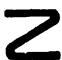
\includegraphics[keepaspectratio]{images/part002_84c4f053.jpg}}


\begin{enumerate}
\def\labelenumi{(\arabic{enumi})}
\setcounter{enumi}{4}
\tightlist
\item
  The powers of any prime ideal are not necessarily primary ideals (Exercise 1). On the other hand, there exist primary ideals which are not powers of prime ideals (Exercise 1).
\end{enumerate}

PROPOSITION 2. Let M be a module over a Noetherian ring A, p a prime ideal of A and \((Q_{i})_{i\in I}\) a non-empty finite family of submodules of M which are p-primary with respect to M. Then \(\bigcap_{i\in I} Q_{i}\) is p-primary with respect to M.

\(\mathrm{M}/\left(\bigcap_{i\in\mathrm{I}}\mathrm{Q}_{i}\right)\) is isomorphic to a submodule \(\neq0\) of the direct sum \(\bigoplus_{i\in\mathrm{I}}(\mathrm{M}/\mathrm{Q}_{i})\) . Now

\[
\operatorname{Ass} \left(\bigoplus_ {i \in I} (M / Q _ {i})\right) = \bigcup_ {i \in I} \operatorname{Ass} (M / Q _ {i}) = \{p \}
\]

(§ 1, no. 1, Corollary 1 to Proposition 3). Hence \(\operatorname{Ass}\left(M / \left(\bigcap_{i \in I} Q_i\right)\right) = \{p\}\) (§ 1, no. 1, Proposition 3 and Corollary 1 to Proposition 2).

PROPOSITION 3. Let A be a Noetherian ring, S a multiplicative subset of A, p a prime ideal of A, M an A-module, N a submodule of M and \(i = i_{A}^{S}\) the canonical mapping of M to \(S^{-1}M\) .

\begin{enumerate}
\def\labelenumi{(\roman{enumi})}
\item
  Suppose that \(\mathfrak{p} \cap \mathbf{S} \neq \varnothing\) . If \(\mathbf{N}\) is \(\mathfrak{p}\) -primary with respect to \(\mathbf{M}\) , then \(\mathbf{S}^{-1}\mathbf{N} = \mathbf{S}^{-1}\mathbf{M}\) .
\item
  Suppose that \(\mathfrak{p} \cap \mathbf{S} = \varnothing\) . For \(\mathbf{N}\) to be \(\mathfrak{p}\) -primary with respect to \(\mathbf{M}\) , it is necessary and sufficient that \(\mathbf{N}\) be of the form \(i^{-1}(\mathbf{N}')\) , where \(\mathbf{N}'\) is a sub- \(\mathbf{S}^{-1}\mathbf{A}\) -module of \(\mathbf{S}^{-1}\mathbf{M}\) which is \((\mathbf{S}^{-1}\mathfrak{p})\) -primary with respect to \(\mathbf{S}^{-1}\mathbf{M}\) ; then \(\mathbf{N}' = \mathbf{S}^{-1}\mathbf{N}\) .
\item
  If \(\mathfrak{p} \cap S \neq \varnothing\) and \(N\) is \(\mathfrak{p}\) -primary with respect to \(M\) , then
\end{enumerate}

\[
\mathrm{Ass} _ {\mathbf {S} ^ {- 1} \mathbf {A}} (\mathrm{S} ^ {- 1} (\mathrm{M} / \mathrm{N})) = \varnothing
\]

(§ 1, no. 2, Corollary to Proposition 5) and hence \(S^{-1}(M/N) = 0\) (§ 1, no. 1, Corollary 1 to Proposition 2), whence \(S^{-1}M/S^{-1}N = 0\) .

\begin{enumerate}
\def\labelenumi{(\roman{enumi})}
\setcounter{enumi}{1}
\tightlist
\item
  Suppose that \(\mathfrak{p} \cap \mathrm{S} = \varnothing\) . If \(\mathbf{N}\) is \(\mathfrak{p}\) -primary with respect to \(\mathbf{M}\) , then \(\operatorname{Ass}_{\mathbf{S}^{-1}\mathbf{A}}(\mathrm{S}^{-1}(\mathrm{M/N})) = \{\mathrm{S}^{-1}\mathfrak{p}\}\) ( \(\S 1\) , no. 2, Corollary to Proposition 5) and hence the submodule \(\mathbf{N}' = \mathrm{S}^{-1}\mathbf{N}\) of \(\mathrm{S}^{-1}\mathbf{M}\) is \((\mathrm{S}^{-1}\mathfrak{p})\) -primary; moreover, if \(s \in \mathbf{S}\) and \(m \in \mathbf{M}\) are such that \(sm \in \mathbf{N}\) , then \(m \in \mathbf{N}\) , for the homothety with ratio \(s\) in \(\mathbf{M/N}\) is injective, whence \(\mathbf{N} = \overline{i}^{1}(\mathbf{N}')\) (Chapter II, \(\S 2\) , no. 4, Proposition 10). Conversely, let \(\mathbf{N}'\) be a submodule of \(\mathrm{S}^{-1}\mathbf{M}\) which is \((\mathrm{S}^{-1}\mathfrak{p})\) -primary with respect to \(\mathrm{S}^{-1}\mathbf{M}\) ; let us write \(\mathbf{N} = \overline{i}^{1}(\mathbf{N}')\) ; then \(\mathbf{N}' = \mathrm{S}^{-1}\mathbf{N}\) (Chapter II, \(\S 2\) , no. 4, Proposition 10) and \(\operatorname{Ass}_{\mathbf{S}^{-1}\mathbf{A}}(\mathrm{S}^{-1}(\mathrm{M/N})) = \operatorname{Ass}_{\mathbf{S}^{-1}\mathbf{A}}((\mathrm{S}^{-1}\mathbf{M})/\mathrm{N}') = \{\mathrm{S}^{-1}\mathfrak{p}\}\) . As the canonical mapping \(\mathrm{M/N} \to \mathrm{S}^{-1}(\mathrm{M/N})\) is injective, no prime ideal of \(\mathbf{A}\) associated with \(\mathbf{M/N}\) meets \(\mathbf{S}\) ( \(\S 1\) , no. 2, Proposition 6); it follows that \(\operatorname{Ass}(\mathrm{M/N}) = \{\mathfrak{p}\}\) ( \(\S 1\) , no. 2, Corollary to Proposition 5), so that \(\mathbf{N}\) is \(\mathfrak{p}\) -primary with respect to \(\mathbf{M}\) .
\end{enumerate}

\subsection{The existence of a primary decomposition}

DEFINITION 2. Let A be a Noetherian ring, M an A-module and N a submodule of M. A finite family \((\mathbf{Q}_i)_{i\in I}\) of submodules of M which are primary with respect to M and such that \(\mathbf{N} = \bigcap_{i\in I}\mathbf{Q}_i\) is called a primary decomposition of N in M.

Example. Let us take \(\mathbf{A} = \mathbf{Z}\) , \(\mathbf{M} = \mathbf{Z}\) , \(\mathbf{N} = n\mathbf{Z}\) for some integer \(n > 0\) . If \(n = p_{1}^{\alpha_1} \ldots p_{k}^{\alpha_k}\) is the decomposition of \(n\) into prime factors,

\[
n \mathbf {Z} = (p _ {1} ^ {\alpha_ {1}} \mathbf {Z}) \cap \dots \cap (p _ {k} ^ {\alpha_ {k}} \mathbf {Z})
\]

is a primary decomposition of \(n\mathbf{Z}\) in \(\mathbf{Z}\) by Example 4 of no. 1.

By an abuse of language, the relation \(\mathbf{N} = \bigcap_{i \in I} \mathbf{Q}_i\) is called a primary decomposition of \(\mathbf{N}\) in \(\mathbf{M}\) . It amounts to the same to say that \(\{0\} = \bigcap_{i \in I} (\mathbf{Q}_i / \mathbf{N})\) is a primary decomposition of \(\{0\}\) in \(\mathbf{M} / \mathbf{N}\) . If \((\mathbf{Q}_i)_{i \in I}\) is a primary decomposition of \(\mathbf{N}\) in \(\mathbf{M}\) , the canonical mapping from \(\mathbf{M} / \mathbf{N}\) to \(\bigoplus_{i \in I} (\mathbf{M} / \mathbf{Q}_i)\) is injective. Conversely let \(\mathbf{N}\) be a submodule of \(\mathbf{M}\) and \(f\) an injective homomorphism from \(\mathbf{M} / \mathbf{N}\) to a finite direct sum \(\mathbf{P} = \bigoplus_{i \in I} \mathbf{P}_i\) , where each set \(\operatorname{Ass}(\mathbf{P}_i)\) is reduced to a single element \(p_i\) ; let \(f_i\) be the homomorphism \(\mathbf{M} / \mathbf{N} \to \mathbf{P}_i\) obtained by taking the composition of \(f\) with the projection \(\mathbf{P} \to \mathbf{P}_i\) and let \(Q_i / \mathbf{N}\) be the kernel of \(f_i\) ; then the \(Q_i\) distinct from \(\mathbf{M}\) are primary with respect to \(\mathbf{M}\) (no. 1, Definition 1) and \(\mathbf{N} = \bigcap_{i \in I} Q_i\) . Moreover, \(\operatorname{Ass}(\mathbf{M} / \mathbf{N}) \subset \bigcup_{i \in I} \{\mathfrak{p}_i\}\) by virtue of § 1, no. 1, Proposition 3.

THEOREM 1. Let M be a finitely generated module over a Noetherian ring and let N be a submodule of M. There exists a primary decomposition of N of the form

\[
N = \bigcap_ {\mathfrak {p} \in \operatorname{Ass} (M / N)} Q (\mathfrak {p})\tag{1}
\]

where, for all \(\mathfrak{p} \in \operatorname{Ass}(\mathbf{M} / \mathbf{N})\) , \(\mathbf{Q}(\mathfrak{p})\) is \(\mathfrak{p}\) -primary with respect to \(\mathbf{M}\) .

We may replace M by M/N and therefore suppose that N = 0. By § 1, no. 4, Corollary to Theorem 2, Ass(M) is finite; by § 1, no. 1, Proposition 4, there exists, for each \(p \in \text{Ass}(M)\) , a submodule \(Q(p)\) of M such that \(\text{Ass}(M/Q(p)) = \{p\}\) and \(\text{Ass}(Q(p)) = \text{Ass}(M) - \{p\}\) . Let us write \(P = \bigcap_{p \in \text{Ass}(M)} Q(p)\) ; for all \(p \in \text{Ass}(M)\) , \(\text{Ass}(P) \subset \text{Ass}(Q(p))\) and hence \(\text{Ass}(P) = \varnothing\) , which implies P = 0 (§ 1, no. 1, Corollary 1 to Proposition 2) and therefore proves the theorem.

\subsection{Uniqueness properties in the primary decomposition}

DEFINITION 3. Let M be a module over a Noetherian ring and N a submodule of M. A primary decomposition \(N = \bigcap_{i \in I} Q_i\) of N in M is called reduced if the following conditions are fulfilled:

\begin{enumerate}
\def\labelenumi{(\alph{enumi})}
\item
  there exists no index \(i \in \mathbf{I}\) such that \(\bigcap_{j \neq i} Q_j \subset Q_i\) ;
\item
  if \(\operatorname{Ass}(\mathbf{M} / \mathbf{Q}_i) = \{\mathfrak{p}_i\}\) , the \(\mathfrak{p}_i\) ( \(i \in \mathbf{I}\) ) are distinct.
\end{enumerate}

From every primary decomposition \(\mathbf{N} = \bigcap_{i\in \mathbf{I}}\mathbf{Q}_i\) of \(\mathbf{N}\) in \(\mathbf{M}\) a reduced primary decomposition of \(\mathbf{M}\) in \(\mathbf{N}\) can be deduced as follows: let \(\mathbf{J}\) be a minimal element of the set of subsets \(\mathbf{I}'\) of \(\mathbf{I}\) such that \(\mathbf{N} = \bigcap_{i\in \mathbf{I}'}\mathbf{Q}_i\) . Clearly \((\mathbf{Q}_i)_{i\in \mathbf{J}}\) satisfies condition (a). Then let \(\Phi\) be the set of \(p_i\) for \(i\in J\) ; for all \(p\in \Phi\) , let \(H(p)\) be the set of \(i\in J\) such that \(p_i = p\) and let \(Q(p) = \bigcap_{i\in H(p)}Q_i\) ; it follows from Proposition 2 of no. 1 that \(Q(p)\) is \(p\) -primary with respect to \(M\) ; further \(N = \bigcap_{p\in \Phi}Q(p)\) and the family \(Q((p))_{p\in \Phi}\) is therefore a reduced primary decomposition of \(N\) in \(M\) . We shall see that the primary decomposition defined in the proof of Theorem 1 of no. 2 is reduced; this follows from the following proposition:

PROPOSITION 4. Let M be a module over a Noetherian ring, N a submodule of M, \(N = \bigcap_{i \in I} Q_i\) a primary decomposition of N in M and, for all \(i \in I\) , let \(\{p_i\} = \text{Ass}(M/Q_i)\) . For this decomposition to be reduced, it is necessary and sufficient that the \(p_i\) be distinct and belong to \(\text{Ass}(M/N)\) ; then

\begin{enumerate}
\def\labelenumi{(\arabic{enumi})}
\setcounter{enumi}{1}
\tightlist
\item
\end{enumerate}

\[
\operatorname{Ass} (\mathbf {M} / \mathbf {N}) = \bigcup_ {i \in I} \left\{\mathfrak {p} _ {i} \right\}\tag{3}
\]

\[
\operatorname{Ass} \left(\mathrm{Q} _ {i} / \mathrm{N}\right) = \bigcup_ {j \neq i} \left\{\mathfrak {p} _ {j} \right\} \quad \text{for all } i \in \mathrm{I}.
\]

If the condition of the statement is fulfilled, \(N = \bigcap_{j \neq i} Q_j\) cannot hold, for we would deduce that \(\text{Ass}(M/N) \subset \bigcup_{j \neq i} \{p_j\}\) (§ 1, no. 1, Corollary 2 to Proposition 3) contrary to the hypothesis; the primary decomposition \((Q_i)_{i \in I}\) of N is then certainly reduced. Conversely, \(\text{Ass}(M/N) \subset \bigcup_{i \in I} \{p_i\}\) always holds (§ 1, no. 1, Corollary 2 to Proposition 3); on the other hand, for all \(i \in I\) , let us write \(P_i = \bigcap_{j \neq i} Q_j\) ; then \(P_i \cap Q_i = N\) and \(P_i \neq N\) if \((Q_i)_{i \in I}\) is reduced, hence \(P_i/N\) is non-zero and is isomorphic to the submodule \((P_i + Q_i)/Q_i\) of \(M/Q_i\), whence \(\{p_i\} = \text{Ass}(P_i/N)\) (§ 1, no. 1, Proposition 3 and Corollary 1 to Proposition 2); as \(P_i/N \subset M/N\) , \(p_i \in \text{Ass}(M/N)\) , which completes the proof of the necessity of the condition in the statement and formula (2). Finally, as \(N = \bigcap_{j \neq i} (Q_j \cap Q_i)\) , \(\text{Ass}(Q_i/N) \subset \bigcup_{j \neq i} \text{Ass}(Q_i/(Q_j \cap Q_i))\) (§ 1, no. 1, Corollary 2 to Proposition 3); but \(Q_i/(Q_j \cap Q_i)\) is isomorphic to the submodule \((Q_i + Q_j)/Q_j\) of \(M/Q_j\), hence \(\text{Ass}(Q_i/(Q_j \cap Q_i)) \subset \{p_j\}\) and

\[
\operatorname{Ass} \left(Q _ {i} / N\right) \subset \bigcup_ {j \neq i} \left\{\mathfrak {p} _ {j} \right\};
\]

taking account of (2) and Proposition 3 of §1, no. 1, formula (3) follows easily.

COROLLARY. Let A be a Noetherian ring, M an A-module, N a submodule of M and \((\mathbf{Q}_{i})_{i\in I}\) a primary decomposition of N in M. Then \(\operatorname{Card}(\mathbf{I}) \geqslant \operatorname{Card}(\operatorname{Ass}(\mathbf{M}/\mathbf{N}))\) ; for \((\mathbf{Q}_{i})_{i\in I}\) to be a reduced primary decomposition, it is necessary and sufficient that \(\operatorname{Card}(\mathbf{I}) = \operatorname{Card}(\operatorname{Ass}(\mathbf{M}/\mathbf{N}))\) .

It follows from the remarks preceding Proposition 4 that there exists a reduced primary decomposition \((\mathbf{R}_j)_{j\in J}\) of \(N\) in \(M\) such that \(\operatorname{Card}(J) \leqslant \operatorname{Card}(I)\) ; the first assertion then follows from the second and the latter is a consequence of Proposition 4.

PROPOSITION 5. Let A be a Noetherian ring, M an A-module, N a submodule of M, \(\mathbf{N} = \bigcap_{i \in I} \mathbf{Q}_i\) a reduced primary decomposition of N in M and, for all \(i \in I\) , let \(\{\mathfrak{p}_i\} = \operatorname{Ass}(\mathbf{M} / \mathbf{Q}_i)\) . If \(\mathfrak{p}_i\) is a minimal element of \(\operatorname{Ass}(\mathbf{M} / \mathbf{N})\) , \(\mathbf{Q}_i\) is equal to the saturation on N with respect to \(\mathfrak{p}_i\) (Chapter II, §2, no. 4) (cf.~Exercise 2).

We can obviously restrict our attention to the case where N = 0, replacing if need be M by M/N. If \(p_{i}\) is minimal in Ass(M), the set of elements of Ass(M) which do not meet A - \(p_{i}\) reduces to \(p_{i}\) ; the proposition then follows from formula (3) above and §1, no. 2, Proposition 6, the kernel of the canonical mapping \(M \to M_{p_{i}}\) being equal to the saturation of 0 with respect to \(p_{i}\) (Chapter II, §2, no. 4).

Remark. The prime ideals \(\mathfrak{p}_i\in\mathrm{Ass}(\mathbf{M}/\mathbf{N})\) which are not minimal elements of this set are sometimes called the immersed prime ideals associated with \(\mathbf{M}/\mathbf{N}\) ; if \(\mathbf{M}/\mathbf{N}\) is finitely generated, for \(\mathfrak{p}_0\in\mathrm{Ass}(\mathbf{M}/\mathbf{N})\) to be immersed, it is necessary and sufficient that \(\mathrm{V}(\mathfrak{p}_0)\) be not an irreducible component of \(\mathrm{Supp}(\mathbf{M}/\mathbf{N})\) (Chapter II, § 4, no. 3, Corollary 2 to Proposition 14); if \((\mathrm{Q}(\mathfrak{p}))_{\mathfrak{p}\in\mathrm{Ass}(\mathbf{M}/\mathbf{N})}\) and \((\mathrm{Q}'(\mathfrak{p}))_{\mathfrak{p}\in\mathrm{Ass}(\mathbf{M}/\mathbf{N})}\) are two reduced primary decompositions of \(\mathbf{N}\) in \(\mathbf{M}\) , it may be that \(\mathrm{Q}'(\mathfrak{p}_0)\neq\mathrm{Q}(\mathfrak{p}_0)\) (Exercise 24 (c)); a canonical reduced primary decomposition of \(\mathbf{N}\) in \(\mathbf{M}\) may always be defined by imposing supplementary conditions on the primary submodules which appear in it (Exercise 4).

\subsection{The localization of a primary decomposition}

Given a submodule N of a module M over a Noetherian ring A, to simplify we shall denote by \(D_{I}(M/N)\) , in this no., the set of reduced primary decompositions of N in M whose indexing set is I (equipotent to Ass(M/N)).

PROPOSITION 6. Let A be a Noetherian ring, M an A-module, N a submodule of M and I = Ass(M/N). Let S be a multiplicative subset of A and J the subset of I consisting of the indices \(i\) such that \(\mathbf{S} \cap \mathfrak{p}_i = \varnothing\) . Let \(\mathbf{N}'\) be the saturation of \(\mathbf{N}\) with respect to \(\mathbf{S}\) in \(\mathbf{M}\) . Then:

\begin{enumerate}
\def\labelenumi{(\roman{enumi})}
\item
  If \((\mathbf{Q}_i)_{i\in I}\) is an element of \(\mathbf{D}_{\mathrm{I}}(\mathbf{M} / \mathbf{N})\) , the family \((\mathbf{Q}_i)_{i\in J}\) is an element of \(\mathbf{D}_{J}(\mathbf{M} / \mathbf{N}')\) and the family \((\mathbf{S}^{-1}\mathbf{Q}_i)_{i\in J}\) is an element of \(\mathbf{D}_{J}(\mathbf{S}^{-1}\mathbf{M} / \mathbf{S}^{-1}\mathbf{N})\) .
\item
  The mapping \((\mathbf{Q}_i)_{i\in J}\to (\mathbf{S}^{-1}\mathbf{Q}_i)_{i\in J}\) is a bijection of \(\mathrm{D}_{\mathrm{J}}(\mathbf{M} / \mathbf{N}^{\prime})\) onto \(\mathbf{D}_{\mathrm{J}}(\mathbf{S}^{-1}\mathbf{M} / \mathbf{S}^{-1}\mathbf{N})\) .
\item
  If \((\mathbf{Q}_i)_{i\in J}\) is an element of \(\mathbf{D}_{\mathbf{J}}(\mathbf{M} / \mathbf{N}')\) and \((\mathbf{R}_i)_{i\in I}\) an element of \(\mathbf{D}_{\mathbf{I}}(\mathbf{M} / \mathbf{N})\) , the family \((\mathrm{T}_i)_{i\in I}\) such that \(\mathrm{T}_i = \mathrm{Q}_i\) for \(i\in \mathbf{J}\) and \(\mathrm{T}_i = \mathrm{R}_i\) for \(i\in \mathbf{I} - \mathbf{J}\) is an element of \(\mathbf{D}_{\mathbf{I}}(\mathbf{M} / \mathbf{N})\) .
\item
  We know (no. 1, Proposition 3) that for \(i \in J\) , \(S^{-1}Q_{i}\) is primary for \(S^{-1}p_{i}\) and that for \(i \in I - J\) , \(S^{-1}Q_{i} = S^{-1}M\) ; as \(S^{-1}N = \bigcap_{i \in I} S^{-1}Q_{i}\) (Chapter II, § 2, no. 4), then also \(S^{-1}N = \bigcap_{i \in J} S^{-1}Q_{i}\) . The \(S^{-1}p_{i}\) for \(i \in J\) are distinct and their set is \(\operatorname{Ass}(S^{-1}M / S^{-1}N)\) (§ 1, no. 2, Corollary to Proposition 5); then (Proposition 4) ( \(S^{-1}Q_{i})_{i \in J}\) is a reduced primary decomposition of \(S^{-1}N\) . Moreover, \(Q_{i} = (i_{M}^{S})^{-1}(S^{-1}Q_{i})\) (no. 1 Proposition 3), hence \(N' = (i_{M}^{S})^{-1}(S^{-1}N) = \bigcap_{i \in J} Q_{i}\) and \((Q_{i})_{i \in J}\) is obviously a reduced primary decomposition of \(N'\) in M.
\item
  As \(S^{-1}N' = S^{-1}N\) , we may replace N by \(N'\) , that is suppose that J = I. Let \((P_i)_{i \in I}\) be a reduced primary decomposition of \(S^{-1}N\) in \(S^{-1}M\) and let us write \(Q_i = (i_M^S)^{-1}(P_i)\) ; it follows from no. 1, Proposition 3 that \(Q_i\) is primary for \(p_i (i \in I)\) and \((Q_i)_{i \in I}\) is then a reduced primary decomposition of N in M by virtue of no. 3, Corollary to Proposition 4. Finally, as, for all \(i \in I\) and every submodule \(Q'_i\) of which M is \(p_i\) -primary with respect to M, \(Q'_i = (i_M^S)^{-1}(S^{-1}Q'_i)\) by virtue of no. 1, Proposition 3 and the hypothesis J = I, we see that two mappings \(D_I(M/N) \to D_I(S^{-1}M/S^{-1}N)\) and \(D_I(S^{-1}M/S^{-1}N) \to D_I(M/N)\) have been defined whose compositions are the identities on \(D_I(M/N)\) and \(D_I(S^{-1}M/S^{-1}N)\) , which proves (ii).
\item
  By virtue of (i), \(\mathbf{N}' = \bigcap_{i\in J}\mathbb{R}_i\) , whence
\end{enumerate}

\[
\mathrm{N} = \mathrm{N} ^ {\prime} \cap \bigcap_ {i \in \mathrm{I} - J} \mathrm{R} _ {i} = \left(\bigcap_ {i \in J} \mathrm{Q} _ {i}\right) \cap \left(\bigcap_ {i \in \mathrm{I} - J} \mathrm{R} _ {i}\right)
\]

and it follows immediately from no. 3, Corollary to Proposition 4 that this primary decomposition is reduced.

COROLLARY. The mappings

\[
\mathrm{D} _ {\mathrm{I}} (\mathrm{M} / \mathrm{N}) \rightarrow \mathrm{D} _ {\mathrm{J}} (\mathrm{M} / \mathrm{N} ^ {\prime}) \quad \text{and} \quad \mathrm{D} _ {\mathrm{I}} (\mathrm{M} / \mathrm{N}) \rightarrow \mathrm{D} _ {\mathrm{J}} (\mathrm{S} ^ {- 1} \mathrm{M} / \mathrm{S} ^ {- 1} \mathrm{N})
\]

defined in Proposition 6 (i) are surjective.

Proposition 6 (iii) shows that the mapping \(\mathrm{D}_{\mathrm{I}}(\mathrm{M}/\mathrm{N}) \rightarrow \mathrm{D}_{\mathrm{J}}(\mathrm{M}/\mathrm{N}')\) is surjective and Proposition 6 (ii) then shows that the mapping

\[
\mathrm{D} _ {\mathrm{I}} (\mathrm{M} / \mathrm{N}) \rightarrow \mathrm{D} _ {\mathrm{J}} (\mathrm{S} ^ {- 1} \mathrm{M} / \mathrm{S} ^ {- 1} \mathrm{N})
\]

is surjective.

\subsection{Rings and modules of finite length}

If an A-module M is of finite length, we shall denote this length by \(\text{long}_{\mathbf{A}}(\mathbf{M})\) or \(\text{long}(\mathbf{M})\) . Recall that every Artinian ring is Noetherian (Algebra, Chapter VIII, § 6, no. 5, Corollary 3 to Proposition 12) and that every finitely generated module over an Artinian ring is of finite length (loc. cit., Corollary 1 to Proposition 12). Moreover, every Artinian integral domain is a field (Algebra, Chapter VIII, § 6, no. 4, Proposition 9).

PROPOSITION 7. Let M be a finitely generated module over a Noetherian ring A. The following properties are equivalent:

\begin{enumerate}
\def\labelenumi{(\alph{enumi})}
\item
  M is of finite length.
\item
  Every ideal \(\mathfrak{p} \in \operatorname{Ass}(\mathbf{M})\) is a maximal ideal of \(\mathbf{A}\) .
\item
  Every ideal \(\mathfrak{p} \in \operatorname{Supp}(\mathbf{M})\) is a maximal ideal of \(\mathbf{A}\) .
\end{enumerate}

Let \((\mathbf{M}_i)_{0\leqslant i\leqslant n}\) be a composition series of M such that, for \(0\leqslant i\leqslant n - 1\) , \(\mathbf{M}_i / \mathbf{M}_{i + 1}\) is isomorphic to \(\mathrm{A} / \mathfrak{p}_i\) , where \(\mathfrak{p}_i\) is prime (§ 1, no. 4, Theorem 1). If M is of finite length, so is each of the A-modules \(\mathrm{A} / \mathfrak{p}_i\) , which implies that each of the rings \(\mathrm{A} / \mathfrak{p}_i\) is Artinian; but as \(\mathrm{A} / \mathfrak{p}_i\) is an integral domain, it is therefore a field, in other words \(\mathfrak{p}_i\) is maximal; we conclude that (a) implies (b) (§ 1, no. 4, Theorem 2). Condition (b) implies (c) by § 1, no. 3, Proposition 7. Finally, if all the ideals of \(\operatorname {Supp}(\mathbf{M})\) are maximal, so are the \(\mathfrak{p}_i\) (§ 1, no. 4, Theorem 2), hence the \(\mathrm{A} / \mathfrak{p}_i\) are simple A-modules and M is of finite length, which completes the proof.

COROLLARY 1. For every module of finite length M over a Noetherian ring A, \(\operatorname{Ass}(\mathbf{M}) = \operatorname{Supp}(\mathbf{M})\) .

Every element of \(\operatorname{Supp}(\mathbf{M})\) is then minimal in \(\operatorname{Supp}(\mathbf{M})\) and the conclusion follows from § 1, no. 3, Corollary 1 to Proposition 7.

COROLLARY 2. Let M be a finitely generated module over a Noetherian ring A and p a prime ideal of A. For \(M_{p}\) to be a non-zero \(A_{p}\) -module of finite length, it is necessary and sufficient that p be a minimal element of Ass(M).

By § 1, no. 2, Corollary to Proposition 5, \(\operatorname{Ass}_{\mathbf{A}_{\mathfrak{p}}}(\mathbf{M}_{\mathfrak{p}})\) is the set of ideals \(q_{\mathfrak{p}}\) , where \(q\) runs through the set of ideals of \(\operatorname{Ass}(\mathbf{M})\) which are contained in \(p\) . On the other hand, \(p_{\mathfrak{p}}\) is the unique maximal ideal of \(\mathbf{A}_{\mathfrak{p}}\) ; by Proposition 7, for \(\mathbf{M}_{\mathfrak{p}}\) to be an \(\mathbf{A}_{\mathfrak{p}}\) -module of finite length, it is necessary and sufficient that no element of \(\operatorname{Ass}(\mathbf{M})\) be strictly contained in \(p\) . On the other hand, for \(\mathbf{M}_{\mathfrak{p}} \neq 0\) , it is necessary and sufficient by definition that \(\mathfrak{p} \in \operatorname{Supp}(\mathbf{M})\) (Chapter II, § 4, no. 4), that is that \(\mathfrak{p}\) contain an element of \(\operatorname{Ass}(\mathbf{M})\) (§ 1, no. 3, Proposition 7). This proves the corollary.

Remark (1). Let M be a finitely generated module over a Noetherian ring A; let \((\mathbf{M}_{i})_{0\leqslant i\leqslant n}\) be a composition series of M such that, for \(0\leqslant i\leqslant n-1\) , \(M_{i}/M_{i+1}\) is isomorphic to \(A/p_{i}\) , where \(p_{i}\) is a prime ideal of A (§ 1, no. 4, Theorem 1). If p is a minimal element of Ass(M), the length \(\text{long}_{A_{p}}(M_{p})\) is equal to the number of indices i such that \(p_{i}=p\) . For the \((\mathbf{M}_{i})_{p}\) form a composition series of \(M_{p}\) and \((\mathbf{M}_{i})_{p}/(\mathbf{M}_{i+1})_{p}\) is isomorphic to \((\mathbf{A}/p_{i})_{p}\) and hence to \(\{0\}\) if \(p_{i}\neq p\) (since p is minimal in the set of \(p_{i}\) by § 1, no. 4, Theorem 2) and to \((\mathbf{A}/p)_{p}\) which is a field, if \(p_{i}=p\) .

PROPOSITION 8. Let M be a module of finite length over a Noetherian ring A.

\begin{enumerate}
\def\labelenumi{(\roman{enumi})}
\item
  There only exists a single primary decomposition of \(\{0\}\) with respect to \(\mathbf{M}\) indexed by \(\operatorname{Ass}(\mathbf{M})\) (necessarily reduced); let \(\{0\} = \bigcap_{\mathfrak{p} \in \operatorname{Ass}(\mathbf{M})} \mathbf{Q}(\mathfrak{p})\) be this decomposition, where \(\mathbf{Q}(\mathfrak{p})\) is \(\mathfrak{p}\) -primary with respect to \(\mathbf{M}\) .
\item
  There exists an integer \(n_0\) such that, for all \(n \geqslant n_0\) and all \(\mathfrak{p} \in \operatorname{Ass}(\mathbf{M})\) , \(\mathbf{Q}(\mathfrak{p}) = \mathfrak{p}^n\mathbf{M}\) .
\item
  For all \(\mathfrak{p} \in \operatorname{Ass}(\mathbf{M})\) , the canonical mapping of \(\mathbf{M}\) to \(\mathbf{M}_{\mathfrak{p}}\) is surjective and its kernel is \(\mathbf{Q}(\mathfrak{p})\) .
\item
  The canonical injection of \(\mathbf{M}\) into \(\bigoplus_{\mathfrak{p} \in \mathbf{Ass}(\mathbf{M})} (\mathbf{M} / \mathbf{Q}(\mathfrak{p}))\) is bijective.
\end{enumerate}

As every element \(\mathfrak{p} \in \operatorname{Ass}(M)\) is minimal in \(\operatorname{Ass}(M)\) (Proposition 7), assertion (i) follows from no. 3, Proposition 5. As \(M\) is finitely generated, there exists \(n_0\) such that \(\mathfrak{p}^n M \subset Q(\mathfrak{p})\) for all \(\mathfrak{p} \in \operatorname{Ass}(M)\) and all \(n \geqslant n_0\) (no. 1, Remark); but as \(\mathfrak{p}\) is a maximal ideal, \(\mathfrak{p}^n M\) is \(\mathfrak{p}\) -primary with respect to \(M\) (no. 1, Examples 2 and 3) and, as \(\bigcap_{\mathfrak{p} \in \operatorname{Ass}(M)} \mathfrak{p}^n M = \{0\}\) , it follows from (i) that necessarily \(\mathfrak{p}^n M = Q(\mathfrak{p})\) for all \(\mathfrak{p} \in \operatorname{Ass}(M)\) ; whence (ii). As the \(\mathfrak{p}^n\) , for \(\mathfrak{p} \in \operatorname{Ass}(M)\) , are relatively prime in pairs (Chapter II, § 1, no. 2, Proposition 3), the canonical mapping \(M \to \bigoplus_{\mathfrak{p} \in \operatorname{Ass}(M)} (M / \mathfrak{p}^n M)\) is surjective (Chapter II, § 1, no. 2, Proposition 6), whence (iv). Then \(\operatorname{Ass}(Q(\mathfrak{p})) = \operatorname{Ass}(M) - \{\mathfrak{p}\}\) and \(\operatorname{Ass}(M / Q(\mathfrak{p})) = \{\mathfrak{p}\}\) (no. 3, Proposition 4); as the elements of \(\operatorname{Ass}(M)\) are maximal ideals, \(\mathfrak{p}\) is the only element of \(\operatorname{Ass}(M)\) which does not meet \(A - \mathfrak{p}\) ; \(Q(\mathfrak{p})\) is therefore the kernel of the canonical mapping \(j: M \to M_{\mathfrak{p}}\) (§ 1, no. 2, Proposition 6). If \(s \in A - \mathfrak{p}\) , the homothety of \(M / Q(\mathfrak{p})\) with ratio \(s\) is injective by virtue of the relation \(\operatorname{Ass}(M / Q(\mathfrak{p})) = \{\mathfrak{p}\}\) (no. 1, Proposition 1); since \(M / Q(\mathfrak{p})\) is Artinian, this homothety is bijective (Algebra, Chapter VIII, § 1, no. 2, Lemma 3). The canonical mapping \(M \to M / Q(\mathfrak{p})\) is then written \(f \circ j\) , where \(f: M_{\mathfrak{p}} \to M / Q(\mathfrak{p})\) is an A-homomorphism (Chapter II, § 2, no. 2, Proposition 3); as \(\operatorname{Ker}(j) = \operatorname{Ker}(f \circ j) = Q(\mathfrak{p})\) , \(f\) is injective; we conclude that \(j\) is surjective and \(f\) bijective.

COROLLARY. If M is a module of finite length over a Noetherian ring A, then

\[
\operatorname{long} _ {\mathbf {A}} (\mathbf {M}) = \sum_ {\mathfrak {p} \in \mathbf {A s s} (\mathbf {M})} \operatorname{long} _ {\mathbf {A p}} (\mathbf {M} _ {\mathfrak {p}}).\tag{4}
\]

This will follow from Proposition 8 (iv) if we prove that

\[
\operatorname{long} _ {\mathbf {A}} (\mathbf {M} / \mathbf {Q} (\mathfrak {p})) = \operatorname{long} _ {\mathbf {A} _ {\mathfrak {p}}} (\mathbf {M} _ {\mathfrak {p}}).
\]

Now, it follows from Proposition 1 of no. 1 that for all \(s \in \mathbf{A} - \mathfrak{p}\) the homothety with ratio \(s\) on \(\mathrm{M} / \mathrm{Q}(\mathfrak{p})\) is injective; the homothety with ratio \(s\) on every submodule \(\mathbf{R}\) of \(\mathrm{M} / \mathrm{Q}(\mathfrak{p})\) is therefore injective and, as \(\mathbf{R}\) is Artinian, it is bijective (Algebra, Chapter VIII, §2, no. 2, Lemma 3); we conclude that the sub- \(\mathbf{A}\) -modules of \(\mathrm{M} / \mathrm{Q}(\mathfrak{p})\) are the images under the bijection \(f: \mathbf{M}_{\mathfrak{p}} \to \mathbf{M} / \mathbf{Q}(\mathfrak{p})\) of the sub- \(\mathbf{A}_{\mathfrak{p}}\) -modules of \(\mathbf{M}_{\mathfrak{p}}\) (Chapter II, §2, no. 3), whence our assertion.

PROPOSITION 9. Let A be a Noetherian ring. The following conditions are equivalent:

\begin{enumerate}
\def\labelenumi{(\alph{enumi})}
\item
  A is Artinian.
\item
  All the prime ideals of \(\mathbf{A}\) are maximal ideals.
\item
  All the elements of Ass(A) are maximal ideals.
\end{enumerate}

If these conditions are fulfilled, A has only a finite number of prime ideals, which are all maximal and associated with the A-module A; further, A is a semi-local ring and its Jacobson radical is nilpotent.

To say that A is Artinian is equivalent to saying that A is an A-module of finite length; hence (a) and (c) are equivalent by Proposition 7. Clearly (b) implies (c). Finally, (a) implies (b) since every Artinian integral domain is a field. The properties (a), (b) and (c) are therefore equivalent.

Suppose they hold. As every prime ideal of A belongs to Supp(A) and every element of Supp(A) contains an element of Ass(A) (§ 1, no. 3, Proposition 7), it follows from (c) that Ass(A) is the set of all prime ideals of A; then A has only a finite number of prime ideals, all of them maximal and associated with the A-module A. This obviously implies that A is semi-local; finally, we know that the Jacobson radical of an Artinian ring is nilpotent (Algebra, Chapter VIII, § 6, no. 4, Theorem 3).

Remark (2) The conditions of Proposition 9 for a Noetherian ring A imply that the spectrum of A is finite and discrete, every point of \(\operatorname{Spec}(A)\) being therefore closed (Chapter II, §4, no. 3, Corollary 6 to Proposition 11). Conversely, for a Noetherian ring A, to say that every point of \(\operatorname{Spec}(A)\) is closed means that every prime ideal of A is maximal (loc. cit.) and hence this condition is equivalent to that of Proposition 9.

COROLLARY 1. Every Artinian ring A is isomorphic to the direct composition of a finite family of Artinian local rings.

It follows from Proposition 9 and Proposition 8 (iii) and (iv) that, if \((\mathfrak{m}_i)_{1\leqslant i\leqslant n}\) is the family of maximal ideals of A, the canonical mapping \(\mathbf{A}\to \prod_{i}\mathbf{A}_{m_i}\) is bijective.

Remark (3). This corollary can also be deduced from the fact that \(\operatorname{Spec}(A)\) is finite and discrete and Chapter II, § 4, no. 3, Proposition 15.

COROLLARY 2. Let A be a Noetherian ring and m an ideal of A. The following conditions are equivalent:

\begin{enumerate}
\def\labelenumi{(\alph{enumi})}
\item
  A is a semi-local ring and m is a defining ideal of A.
\item
  A is a Zariski ring with the m-adic topology and A/m is Artinian.
\end{enumerate}

If (a) holds, A is a Zariski ring with the m-adic topology (Chapter III, § 3, no. 3, Example 3); further, as by hypothesis m contains a power of the Jacobson radical r of A, every prime ideal of A which contains m also contains r (Chapter II, § 1, no. 1, Proposition 1); it is therefore maximal, since r is a finite intersection of maximal ideals (loc. cit.); Proposition 9 then shows that A/m is Artinian. Conversely, if (b) holds, every maximal ideal p of A contains the Jacobson radical of A and hence contains m (Chapter III, § 3, no. 3, Proposition 6); as A/m is Artinian, the ideals p/m are finite in number (Proposition 9) and hence A has only a finite number of maximal ideals, which implies that it is semi-local.

COROLLARY 3. Let A, A' be two rings and h a homomorphism from A to A'. Suppose that A is semi-local and Noetherian and that A' is a finitely generated A-module. Then the ring A' is semi-local and Noetherian; if m is a defining ideal of A, mA' is a defining ideal of A'.

We know that A' is a Zariski ring with the mA'-adic topology (Chapter III, § 3, no. 3, Proposition 7). As A/m is Artinian (Corollary 2) and A'/mA' is a finitely generated (A/m)-module, A'/mA' is an Artinian ring, hence A' is semi-local and mA' is a defining ideal of A' (Corollary 2).

COROLLARY 4. Let A be a complete semi-local Noetherian ring, m a defining ideal of A, E a finitely generated A-module and \((\mathbf{F}_{n})\) a decreasing sequence of submodules of E such that \(\bigcap_{n} F_{n} = 0\) . Then, for all p \textgreater{} 0, there exists n \textgreater{} 0 such that \(F_{n} \subset m^{p}E\) .

As A is a Zariski ring, E is Hausdorff and the \(F_{n}\) are closed under the m-adic topology. On the other hand, E is complete (Chapter III, § 2, no. 12, Corollary 1 to Proposition 16). Finally, \(E/m^{p}E\) is a finitely generated module over the ring \(A/m^{p}\) , which is Artinian (Corollary 2); then \(E/m^{p}E\) is an Artinian \((A/m^{p})\) -module and hence an Artinian A-module. The corollary then follows from Chapter III, § 2, no. 7, Proposition 8.

COROLLARY 5. In a complete semi-local Noetherian ring every decreasing sequence of ideals whose intersection is 0 is a filter base which converges to 0.

It is sufficient to apply Corollary 4 to the A-module A.

PROPOSITION 10. Let A be a Noetherian ring and \(\mathfrak{p}_1, \ldots, \mathfrak{p}_n\) the prime ideals associated with the A-module A, where \(\mathfrak{p}_i \neq \mathfrak{p}_j\) for \(i \neq j\) .

\begin{enumerate}
\def\labelenumi{(\roman{enumi})}
\item
  The set \(\mathbf{S} = \bigcap_{i=1}^{n} (\mathbf{A} - \mathfrak{p}_i)\) is the set of elements which are not divisors of 0 in A.\\
\item
  If all the \(\mathfrak{p}_i\) are minimal elements of \(\operatorname{Ass}(\mathbf{A})\) , the total ring of fractions \(\mathbf{S}^{-1}\mathbf{A}\) of \(\mathbf{A}\) is Artinian.
\item
  If the ring A is reduced, all the \(p_{i}\) are minimal elements of Ass(A) (and therefore are the minimal elements of Spec(A)) and each of the \(A_{p_{i}}\) is a field; for each index i, the canonical homomorphism \(S^{-1}A \to A_{p_{i}}\) (Chapter II, §2, no. 1, Corollary 1 to Proposition 2) is surjective and its kernel is \(S^{-1}p_{i}\) ; finally the canonical homomorphism from \(S^{-1}A\) to \(\prod_{i=1}^{n} (S^{-1}A/S^{-1}p_{i})\) is bijective.
\end{enumerate}

The fact that S is the set of elements which are not divisors of 0 in A has already been seen ( \(\S\) 1, no. 1, Corollary 3 to Proposition 2). The prime ideals of \(S^{-1}A\) are

of the form \(\mathbf{S}^{-1}\mathfrak{p}\) , where \(\mathfrak{p}\) is a prime ideal of \(\mathbf{A}\) contained in \(\bigcup_{i=1}^{n} \mathfrak{p}_i\) (Chapter II, §2, no. 5, Proposition 10) that is contained in one of the \(\mathfrak{p}_i\) (Chapter II, §1, no. 1, Proposition 2). If \(\mathfrak{p}_i\) is a minimal element of \(\operatorname{Ass}(\mathbf{A})\) , it is a minimal element of \(\operatorname{Spec}(\mathbf{A})\) (§1, no. 3, Corollary to Proposition 7); if each of the \(\mathfrak{p}_i\) is a minimal element of \(\operatorname{Ass}(\mathbf{A})\) , we then see that the prime ideals of \(\mathbf{S}^{-1}\mathbf{A}\) are the \(\mathbf{S}^{-1}\mathfrak{p}_i\) and they are therefore all maximal, which proves that \(\mathbf{S}^{-1}\mathbf{A}\) is Artinian (Proposition 9).

Suppose finally that the ring A is reduced. Then \(\bigcap_{i=1}^{n} p_i = \{0\}\) (§ 1, no. 3,

Corollary 2 to Proposition 7). We deduce that \(\{0\} = \bigcap_{i=1}^{n} p_i\) is a reduced primary decomposition of the ideal \(\{0\}\) (no. 3, Corollary to Proposition 4); in particular, none of the \(p_i\) can contain a \(p_j\) of index \(j \neq i\) and therefore the \(p_i\) are all minimal elements of \(\operatorname{Ass}(A)\) . The ring \(S^{-1}A\) is then Artinian by (ii). The \(S^{-1}p_i\) are prime ideals associated with the \(S^{-1}A\) -module \(S^{-1}A\) ( \(\S\) 1, no. 2, Corollary to Proposition 5) and \(\{0\} = S^{-1}\left(\bigcap_{i=1}^{n} p_i\right) = \bigcap_{i=1}^{n} S^{-1}p_i\) (Chapter II, \(\S\) 2, no. 4); as the \(S^{-1}p_i\) are distinct, \((S^{-1}p_i)_{1 \leqslant i \leqslant n}\) is a reduced primary decomposition of \(\{0\}\) in \(S^{-1}A\) (no. 3, Corollary to Proposition 4). Proposition 8 then shows that the canonical homomorphism \(g_{i} \colon S^{-1}\mathbf{A} \to (\mathbf{S}^{-1}\mathbf{A})_{p_{i}}\) is surjective and has kernel \(S^{-1}p_{i}\) and the canonical homomorphism \(S^{-1}\mathbf{A} \to \prod_{i=1}^{n} (\mathbf{S}^{-1}\mathbf{A}/\mathbf{S}^{-1}p_{i})\) is bijective. We know moreover that the canonical homomorphism \(S^{-1}\mathbf{A} \to A_{p_{i}}\) is composed of \(g_{i}\) and an isomorphism \((\mathbf{S}^{-1}\mathbf{A})_{\mathbf{S}^{-1}p_{i}} \to A_{p_{i}}\) (Chapter II, § 2, no. 3, Proposition 7). Finally, it follows from Proposition 8 that \((\mathbf{S}^{-1}\mathbf{A})_{\mathbf{S}^{-1}p_{i}}\) is isomorphic to \(S^{-1}\mathbf{A}/\mathbf{S}^{-1}p_{i}\) and hence is a field since \(S^{-1}p_{i}\) is a maximal ideal.

\subsection{Primary decomposition and extension of scalars}

In this no., A and B will denote two rings and we shall consider a ring homomorphism \(\rho: \mathbf{A} \to \mathbf{B}\) which makes B into an A-algebra; recall that, for every B-module F, \(\rho_*(\mathbf{F})\) is the commutative group F with the A-module structure defined by \(a.y = \rho(a)y\) for all \(a \in \mathbf{A}, y \in \mathbf{F}\) .

LEMMA 1. Let A be a Noetherian ring, p a prime ideal of A, E an A-module whose annihilator contains a power of p and such that \(\operatorname{Ass}(\mathbf{E}) = \{\mathfrak{p}\}\) and F a B-module such that \(\rho_{*}(\mathbf{F})\) is a flat A-module. The condition \(\mathfrak{P} \in \operatorname{Ass}_{\mathbf{B}}(\mathbf{E} \otimes_{\mathbf{A}} \mathbf{F})\) then implies \(\overline{\rho}^{1}(\mathfrak{P}) = \mathfrak{p}\) .

If \(n\) is such that \(p^n\mathbf{E} = 0\) , then \(p^n\mathbf{B} \subset \operatorname{Ann}(\mathbf{E} \otimes_{\mathbf{A}} \mathbf{F})\) , whence \(p^n\mathbf{B} \subset \mathfrak{P}\) , which implies \(p^n \subset \overline{\rho}^1(\mathfrak{P})\) and therefore \(p \subset \overline{\rho}^1(\mathfrak{P})\) since \(\overline{\rho}^1(\mathfrak{P})\) is prime. Moreover, if \(a \in \mathbf{A} - p\) , the homothety \(h\) with ratio \(a\) on \(\mathbf{E}\) is injective (§ 1, no. 1, Corollary 2 to Proposition 2); as \(h \otimes l_{\mathbf{F}}\) is the homothety \(h'\) with ratio \(\rho(a)\) on \(\mathbf{E} \otimes_{\mathbf{A}} \mathbf{F}\) and \(\rho_*(\mathbf{F})\) is flat, \(h'\) is injective (Chapter I, § 2, no. 2, Definition 1); this proves that \(\rho(a) \notin \mathfrak{P}\) , whence \(\overline{\rho}^1(\mathfrak{P}) = p\) .

THEOREM 2. Let \(\rho: \mathbf{A} \to \mathbf{B}\) be a ring homomorphism, E an A-module and F a B-module such that \(\rho_*(\mathbf{F})\) is a flat A-module. Then

\[
\operatorname{Ass} _ {\mathbf {B}} (\mathrm{E} \otimes_ {\mathbf {A}} \mathrm{F}) \supset \bigcup_ {\mathfrak {p} \in \operatorname{Ass} _ {\mathbf {A}} (\mathrm{E})} \operatorname{Ass} _ {\mathbf {B}} (\mathrm{F} / \mathfrak {p} \mathrm{F}).\tag{5}
\]

When A is Noetherian, the two sides of (5) are equal.

Let \(\mathfrak{p} \in \operatorname{Ass}_{\mathbf{A}}(\mathbf{E})\) ; by definition there exists an exact sequence

\[
0 \rightarrow \mathrm{A} / \mathfrak {p} \rightarrow \mathrm{E}.
\]

Since F is a flat A-module we derive an exact sequence

\[
0 \rightarrow \mathrm{F} / \mathfrak {p} \mathrm{F} \rightarrow \mathrm{E} \otimes_ {\mathrm{A}} \mathrm{F}
\]

whence \(\operatorname{Ass}_{\mathbf{B}}(\mathbf{F} / p\mathbf{F})\subset \operatorname{Ass}_{\mathbf{B}}(\mathbf{E}\otimes_{\mathbf{A}}\mathbf{F})\) , which proves the inclusion (5).

Suppose now that A is Noetherian and let us prove the opposite inclusion.

We proceed in stages:

\begin{enumerate}
\def\labelenumi{(\roman{enumi})}
\tightlist
\item
  Suppose first that E is a finitely generated A-module and that \(\operatorname{Ass}_{\mathbf{A}}(\mathbf{E})\) is reduced to a single element \(p\) . By § 1, no. 4, Theorem 1 there exists a composition series \((\mathrm{E}_i)_{0 \leqslant i \leqslant n}\) of E such that \(\mathrm{E}_i / \mathrm{E}_{i+1}\) is isomorphic to \(\mathbf{A} / p_i\) , where \(p_i\) is a prime ideal of A; moreover (§ 1, no. 4, Theorem 2 and no. 3, Proposition 7) all the \(p_i\) contain \(p\) . As F is a flat A-module, the \(\mathrm{E}_i \otimes_{\mathbf{A}} \mathbf{F}\) form a composition series of \(\mathbf{E} \otimes_{\mathbf{A}} \mathbf{F}\) and \((\mathrm{E}_i \otimes_{\mathbf{A}} \mathbf{F}) / (\mathrm{E}_{i+1} \otimes_{\mathbf{A}} \mathbf{F})\) is identified with
\end{enumerate}

\[
(\mathbf {A} / \mathfrak {p} _ {i}) \otimes_ {\mathbf {A}} \mathbf {F} = \mathbf {F} / \mathfrak {p} _ {i} \mathbf {F}.
\]

Then by virtue of § 1, no. 1, Proposition 3

\[
\operatorname{Ass} _ {\mathbf {B}} (\mathrm{E} \otimes_ {\mathbf {A}} \mathrm{F}) \subset \bigcup_ {i = 0} ^ {n - 1} \operatorname{Ass} _ {\mathbf {B}} (\mathrm{F} / p _ {i} \mathrm{F}).
\]

We know that E is annihilated by a power of p (no. 1, Remark); Lemma 1 then shows that, for all \(\mathfrak{P} \in \operatorname{Ass}_{\mathbf{B}}(\mathbf{E} \otimes_{\mathbf{A}} \mathbf{F})\) , \(\overline{\rho}^{1}(\mathfrak{P}) = \mathfrak{p}\) . As \(\mathbf{F} / \mathfrak{p}_i \mathbf{F}\) is isomorphic to \((\mathbf{A} / \mathfrak{p}_i) \otimes_{\mathbf{A}} \mathbf{F}\) , \(\overline{\rho}^{1}(\mathfrak{P}') = \mathfrak{p}_i\) for all \(\mathfrak{P}' \in \operatorname{Ass}_{\mathbf{B}}(\mathbf{F} / \mathfrak{p}_i \mathbf{F})\) by Lemma 1, whence \(\operatorname{Ass}_{\mathbf{B}}(\mathbf{E} \otimes_{\mathbf{A}} \mathbf{F}) \cap \operatorname{Ass}(\mathbf{F} / \mathfrak{p}_i \mathbf{F}) = \varnothing\) if \(\mathfrak{p}_i \neq \mathfrak{p}\) , which proves the theorem in the case considered.

\begin{enumerate}
\def\labelenumi{(\roman{enumi})}
\setcounter{enumi}{1}
\tightlist
\item
  Suppose only that E is a finitely generated A-module. Let \(p_{i}\) ( \(1 \leqslant i \leqslant n\) ) be the elements of \(\operatorname{Ass}_{\mathbf{A}}(\mathbf{E})\) and let \(\{0\} = \bigcap_{i=1}^{n} Q_{i}\) be a corresponding reduced primary decomposition (no. 3); E is then isomorphic to a submodule of the direct sum of the \(E_{i} = E/Q_{i}\) and, as F is a flat A-module, \(E \otimes_{A} F\) is isomorphic to a submodule of the direct sum of B-modules \(E_{i} \otimes_{A} F\) . We deduce (§ 1, no. 1, Proposition 3 and Corollary 1 to Proposition 3) that
\end{enumerate}

\[
\operatorname{Ass} _ {\mathbf {B}} (\mathrm{E} \otimes_ {\mathrm{A}} \mathrm{F}) \subset \bigcup_ {i = 1} ^ {n} \operatorname{Ass} _ {\mathbf {B}} (\mathrm{E} _ {i} \otimes_ {\mathrm{A}} \mathrm{F}).
\]

But \(E_{i}\) is a finitely generated A-module such that \(\operatorname{Ass}_{\mathbf{A}}(\mathbf{E}_{i})\) is reduced to a single element \(p_{i}\) (no. 1, Definition 1). By (i), \(\operatorname{Ass}_{\mathbf{B}}(\mathbf{E}_{i} \otimes_{\mathbf{A}} \mathbf{F}) = \operatorname{Ass}_{\mathbf{B}}(\mathbf{F}/p_{i}\mathbf{F})\) , whence the theorem in this case.

\begin{enumerate}
\def\labelenumi{(\roman{enumi})}
\setcounter{enumi}{2}
\tightlist
\item
  General case. The B-module \(E \otimes_{A} F\) is the union of the submodules \(E' \otimes_{A} F\) , where \(E'\) runs through the set of finitely generated submodules of the A-module E. If P belongs to \(\operatorname{Ass}_{\mathbf{B}}(\mathbf{E} \otimes_{\mathbf{A}} \mathbf{F})\) , then there exists a finitely generated submodule \(E'\) of E such that \(\mathfrak{P} \in \operatorname{Ass}_{\mathbf{B}}(\mathbf{E}' \otimes_{\mathbf{A}} \mathbf{F})\) . By (ii), there exists \(\mathfrak{p} \in \operatorname{Ass}_{\mathbf{A}}(\mathbf{E}')\) such that \(\mathfrak{P} \in \operatorname{Ass}_{\mathbf{B}}(\mathbf{F}/\mathfrak{p}\mathbf{F})\) ; as \(\operatorname{Ass}_{\mathbf{A}}(\mathbf{E}') \subset \operatorname{Ass}_{\mathbf{A}}(\mathbf{E})\) , this completes the proof of Theorem 2.
\end{enumerate}

COROLLARY 1. If A is Noetherian and \(\mathfrak{P} \in \operatorname{Ass}_{\mathbf{B}}(\mathbf{E} \otimes_{\mathbf{A}} \mathbf{F})\) , then \(\overline{\rho}^{1}(\mathfrak{P}) \in \operatorname{Ass}_{\mathbf{A}}(\mathbf{E})\) and \(\overline{\rho}^{1}(\mathfrak{P})\) is the only prime ideal \(\mathfrak{p}\) of A such that \(\mathfrak{P} \in \operatorname{Ass}_{\mathbf{B}}(\mathbf{F}/\mathfrak{p}\mathbf{F})\) .

This follows from Theorem 2 and Lemma 1 applied to the case where \(\mathbf{E} = \mathbf{A} / \mathfrak{p}\) .

COROLLARY 2. Suppose that A and B are Noetherian and that B is a flat A-module. Let p be a prime ideal of A, Q ⊂ E a p-primary submodule and P a prime ideal of B. For Q ⊗A B to be a P-primary submodule of E ⊗A B, it is necessary and sufficient that pB be a P-primary ideal of B.

Let us apply Theorem 2 to the A-module E/Q and the B-module B; then \(\operatorname{Ass}_{\mathbf{A}}(\mathrm{E} / \mathrm{Q}) = \{\mathfrak{p}\}\) and \((\mathrm{E} / \mathrm{Q})\otimes_{\mathbf{A}}\mathbf{B}\) is isomorphic to \((\mathrm{E}\otimes_{\mathbf{A}}\mathrm{B}) / (\mathrm{Q}\otimes_{\mathbf{A}}\mathrm{B})\) and hence \(\operatorname{Ass}_{\mathbf{B}}((\mathrm{E}\otimes_{\mathbf{A}}\mathrm{B}) / (\mathrm{Q}\otimes_{\mathbf{A}}\mathrm{B})) = \operatorname{Ass}_{\mathbf{B}}(\mathrm{B} / \mathfrak{p}\mathbf{B})\) . To say that \(\mathbf{Q}\otimes_{\mathbf{A}}\mathbf{B}\) is \(\mathfrak{P}\) -primary in \(\mathrm{E}\otimes_{\mathbf{A}}\mathrm{B}\) therefore means that \(\operatorname{Ass}_{\mathbf{B}}(\mathrm{B} / \mathfrak{p}\mathrm{B})\) is reduced to \(\mathfrak{P}\) , whence the corollary.

Remark. Suppose that A and B are Noetherian. Let \(\mathfrak{P}\) be a prime ideal of B and let \(\mathfrak{p} = \overline{\rho}^{1}(\mathfrak{P})\) ; let us write \(S = A - \mathfrak{p}\) and let \(k(\mathfrak{p}) = S^{-1}(A / \mathfrak{p})\) be the field of fractions of \(A / \mathfrak{p}\) . Since \(\mathfrak{P}\) contains \(\mathfrak{pB}\) , \(\mathfrak{P} / \mathfrak{pB}\) is a prime ideal of \(B / \mathfrak{pB}\) . If \(\rho'\) is the composite homomorphism \(A \xrightarrow{\rho} B \to B / \mathfrak{pB}\) , we know that \(S^{-1}(B / \mathfrak{pB})\) is identified with the ring \((\rho'(S))^{-1}(B / \mathfrak{pB})\) and \(\mathfrak{P}' = S^{-1}(\mathfrak{P} / \mathfrak{pB})\) with an ideal of this ring (Chapter II, § 2, no. 2, Proposition 6); as \(\mathfrak{P} / \mathfrak{pB}\) does not meet \(\rho'(S)\) , \(\mathfrak{P}'\) is a prime ideal of \(S^{-1}(B / \mathfrak{pB})\) (Chapter II, § 2, no. 5, Proposition 11); moreover there are canonical isomorphisms between \(S^{-1}(B / \mathfrak{pB})\) , \(S^{-1}((A / \mathfrak{p}) \otimes_{A} B)\) and \((S^{-1}(A / \mathfrak{p})) \otimes_{A} B = k(\mathfrak{p}) \otimes_{A} B\) ; similarly \(S^{-1}(F / \mathfrak{pF})\) is canonically identified with \(k(\mathfrak{p}) \otimes_{A} F\) . This being so, under the hypotheses of Theorem 2, in order that \(\mathfrak{P} \in \operatorname{Ass}_{B}(E \otimes_{A} F)\) , it is necessary and sufficient that \(\mathfrak{p} \in \operatorname{Ass}_{A}(E)\) and

\[
\mathfrak {P} ^ {\prime} \in \operatorname{Ass} _ {k (\mathfrak {p}) \otimes_ {\mathbf {A}} \mathbf {B}} (k (\mathfrak {p}) \otimes_ {\mathbf {A}} \mathbf {F}).
\]

For by Theorem 2 and its Corollary 1, it amounts to verifying that the conditions

\[
" \mathfrak {P} \in \operatorname{Ass} _ {\mathbf {B}} (\mathrm{F} / \mathfrak {p} \mathrm{F})" \quad \text { and } \quad " \mathfrak {P} ^ {\prime} \in \operatorname{Ass} _ {k (\mathfrak {p}) \otimes_ {\mathbf {A}} \mathbf {B}} (k (\mathfrak {p}) \otimes_ {\mathbf {A}} \mathrm{F})"
\]

are equivalent; but, as B is Noetherian, this follows from § 1, no. 2, Corollary to Proposition 5 and the above identifications.

PROPOSITION 11. Suppose that A and B are Noetherian and that B is a flat A-module. Let E be an A-module and E' a submodule of E such that, for every ideal \(\mathfrak{p} \in \operatorname{Ass}_{\mathbf{A}}(\mathbf{E}/\mathbf{E}')\) , \(\mathfrak{p}\mathbf{B}\) is a prime ideal of B or equal to B. Let \(\mathbf{E}' = \bigcap_{\mathfrak{p} \in \operatorname{Ass}(\mathbf{E}/\mathbf{E}')} \mathbf{Q}(\mathfrak{p})\) be a reduced primary decomposition of \(\mathbf{E}'\) in E, \(\mathbf{Q}(\mathfrak{p})\) being \(\mathfrak{p}\) -primary for all \(\mathfrak{p} \in \operatorname{Ass}(\mathbf{E}/\mathbf{E}')\) .

\begin{enumerate}
\def\labelenumi{(\roman{enumi})}
\item
  If \(\mathfrak{p} \in \operatorname{Ass}(\mathrm{E} / \mathrm{E}')\) and \(\mathfrak{p}\mathbf{B} = \mathbf{B}\) , then \(\mathbf{Q}(\mathfrak{p}) \otimes_{\mathbf{A}} \mathbf{B} = \mathbf{E} \otimes_{\mathbf{A}} \mathbf{B}\) .
\item
  If \(\mathfrak{p} \in \operatorname{Ass}(\mathrm{E} / \mathrm{E}')\) and \(\mathfrak{pB}\) is prime, \(\mathsf{Q}(\mathfrak{p})\) is \(\mathfrak{pB}\) -primary in \(\mathbf{E} \otimes_{\mathbf{A}} \mathbf{B}\) .
\item
  If \(\Phi\) is the set of \(\mathfrak{p} \in \operatorname{Ass}(\mathrm{E} / \mathrm{E}')\) such that \(\mathfrak{pB}\) is prime, then
\end{enumerate}

\[
\mathbf {E} ^ {\prime} \otimes_ {\mathbf {A}} \mathbf {B} = \bigcap_ {\mathfrak {p} \in \Phi} (\mathbf {Q} (\mathfrak {p}) \otimes_ {\mathbf {A}} \mathbf {B})
\]

and this relation is a reduced primary decomposition of \(E^{\prime} \otimes_{A} B\) in \(E \otimes_{A} B\) .

If \(\mathfrak{pB} = \mathbf{B}\) , Theorem 2 applied to \(\mathbf{E} / \mathbf{Q}(\mathfrak{p})\) and \(\mathbf{B}\) shows that

\[
\operatorname{Ass} _ {\mathbf {B}} ((\mathrm{E} / \mathrm{Q} (\mathfrak {p})) \otimes_ {\mathbf {A}} \mathbf {B}) = \varnothing
\]

and, as B is Noetherian and is a flat A-module, we conclude (§ 1, no. 1, Corollary 1 to Proposition 2) that \(\mathbf{Q}(\mathfrak{p}) \otimes_{\mathbf{A}} \mathbf{B} = \mathbf{E} \otimes_{\mathbf{A}} \mathbf{B}\) . Assertion (ii) follows from Corollary 2 to Theorem 2, taking \(\mathfrak{P} = \mathfrak{p}\mathbf{B}\) . Finally the relation \(\mathbf{E}' \otimes_{\mathbf{A}} \mathbf{B} = \bigcap_{\mathfrak{p} \in \Phi} (\mathbf{Q}(\mathfrak{p}) \otimes_{\mathbf{A}} \mathbf{B})\) follows from the fact that B is a flat A-module (Chapter I, § 2, no. 6, Proposition 6); as \(\mathfrak{p} = \overline{\rho}^{1}(\mathfrak{p}\mathbf{B})\) for \(\mathfrak{p} \in \Phi\) (Lemma 1), \(\mathfrak{p}\mathbf{B} \neq \mathfrak{p}'\mathbf{B}\) for two distinct ideals \(\mathfrak{p}, \mathfrak{p}'\) of the set \(\Phi\) ; on the other hand,

\[
\operatorname{Ass} ((\mathbf {E} \otimes_ {\mathbf {A}} \mathbf {B}) / (\mathbf {E} ^ {\prime} \otimes_ {\mathbf {A}} \mathbf {B})) = \Phi
\]

by Theorem 2; we conclude from no. 3, Proposition 4 that

\[
\mathbf {E} ^ {\prime} \otimes_ {\mathbf {A}} \mathbf {B} = \bigcap_ {\mathfrak {p} \in \Phi} (\mathbf {Q} (\mathfrak {p}) \otimes_ {\mathbf {A}} \mathbf {B})
\]

is a reduced primary decomposition.

COROLLARY. Suppose that \(\mathfrak{pB}\) is prime for all \(\mathfrak{p} \in \operatorname{Ass}_{\mathbf{A}}(\mathrm{E}/\mathrm{E}')\) . Then, if \(\mathfrak{p}_1, \ldots, \mathfrak{p}_n\) are the minimal elements of \(\operatorname{Ass}_{\mathbf{A}}(\mathrm{E}/\mathrm{E}')\) , the \(\mathfrak{p}_i\mathbf{B}\) are minimal elements of

\[
\operatorname{Ass} _ {\mathbf {A}} ((\mathbf {E} \otimes_ {\mathbf {A}} \mathbf {B}) / (\mathbf {E} ^ {\prime} \otimes_ {\mathbf {A}} \mathbf {B})).
\]

It follows from Proposition 11 that in this case \(\mathfrak{p}_i\mathbf{B} \neq \mathfrak{p}_j\mathbf{B}\) for \(i \neq j\) .

\textbf{Examples}\par

\begin{enumerate}
\def\labelenumi{(\arabic{enumi})}
\item
  Let us take \(B = S^{-1}A\) , where S is a multiplicative subset of A; if A is Noetherian, the hypotheses of Proposition 11 are satisfied and we recover a part of Proposition 6 of no. 4.
\item
  Let A be a Noetherian ring, m an ideal of A and B the Hausdorff completion of A with respect to the m-adic topology; then B is a flat A-module and Theorem 2 may be applied with F = B; but in general the hypotheses of Proposition 11 are not satisfied for the prime ideals of A (Chapter III, § 2, Exercise 15 (b)).
\item
  Let A be a Noetherian ring and B the polynomial algebra \(A[X_{1},\ldots,X_{n}]\) ; B is Noetherian and is a free A-module and therefore flat. Also, if p is a prime ideal of A, B/pB is isomorphic to \((A/p)[X_{1},\ldots,X_{n}]\) , which is an integral domain, and hence pB is prime; the hypotheses of Proposition 11 are therefore satisfied for every A-module E and every submodule \(E'\) of E.
\item
  Let A be a finitely generated algebra over a field k, K an extension of k and \(B = A \otimes_{k} K\) the algebra over K obtained by extension of scalars; A and B are Noetherian and B is a free A-module and hence Theorem 2 may be applied to F = B. In certain cases (for example if k is algebraically closed) it can be shown that for every prime ideal p of A, pB is prime or equal to B; we shall return later to this example.
\end{enumerate}

\section{PRIMARY DECOMPOSITION IN GRADED MODULES}

\subsection{Prime ideals associated with a graded module}

PROPOSITION 1. Let \(\Delta\) be a torsion-free commutative group, A a graded ring of type \(\Delta\) and M a graded A-module of type \(\Delta\) . Every prime ideal associated with M is graded and is the annihilator of a homogeneous element of M.

We know that \(\Delta\) can be given a total order structure compatible with its group structure (Algebra, Chapter II, § 11, no. 4, Lemma 2). Let p be a prime ideal associated with M, the annihilator of an element \(x \in M\) , and let \((x_{i})_{i \in \Delta}\) be the family of homogeneous components of x; let \(i(1) < i(2) < \cdots < i(r)\) be the values of i for which \(x_{i} \neq 0\) . Consider an element \(a \in p\) and let \((a_{i})_{i \in \Delta}\) be the family of its homogeneous components; we shall prove that \(a_{i} \in p\) for all \(i \in \Delta\) , which will show that p is a graded ideal.

We argue by induction on the number of indices \(i\) such that \(a_{i} \neq 0\) . Our assertion is obvious if this number is 0; if not, let \(m\) be the greatest of the indices \(i\) for which \(a_{i} \neq 0\) ; if we prove that \(a_{m} \in \mathfrak{p}\) , the induction hypothesis applied to \(a - a_{m}\) will give the conclusion. Now, \(ax = 0\) ; for all \(j \in \Delta\) , using the fact that the homogeneous component of degree \(m + j\) of \(ax\) is 0, we obtain \(\sum_{i \in \Delta} a_{m - i} x_{j + i} = 0\) ; we conclude that \(a_{m} x_{j}\) is a linear combination of the \(x_{i}\) of indices \(i > j\) . In particular therefore \(a_{m} x_{i(r)} = 0\) , whence, by descending induction on \(n < r\) , \(a_{m}^{r - n + 1} x_{i(n)} = 0\) . Then \(a_{m}^{r} x = 0\) , whence \(a_{m}^{r} \in \mathfrak{p}\) and, as \(\mathfrak{p}\) is prime, \(a_{m} \in \mathfrak{p}\) .

We now show that \(\mathfrak{p}\) is the annihilator of a homogeneous element of M. Let us write \(\mathfrak{b}_n = \operatorname{Ann}(x_{i(n)})\) for \(1 \leqslant n \leqslant r\) . For every homogeneous element \(b\) of \(\mathfrak{p}\) and all \(n\) the homogeneous component of \(bx\) of degree \(i(n) + \deg(b)\) is \(bx_{i(n)}\) , hence \(bx_{i(n)} = 0\) and therefore \(b \in \mathfrak{b}_n\) ; as \(\mathfrak{p}\) is generated by its homogeneous elements, \(\mathfrak{p} \subset \mathfrak{b}_n\) . On the other hand, clearly \(\bigcap_{n=1}^{r} \mathfrak{b}_n \subset \operatorname{Ann}(x) = \mathfrak{p}\) ; as \(\mathfrak{p}\) is prime, there exists an \(n\) such that \(\mathfrak{b}_n \subset \mathfrak{p}\) (Chapter II, § 1, no. 1, Proposition 1), whence \(\mathfrak{b}_n = \mathfrak{p} = \operatorname{Ann}(x_{i(n)})\) , which completes the proof.

COROLLARY. For every (necessarily graded) prime ideal p associated with a graded A-module M, there exists an index \(k \in \Delta\) such that the graded A-module \((\mathbf{A}/\mathfrak{p})(k)\) obtained from the graded A-module A/p by diminishing the degrees by k (Algebra, Chapter II, § 11, no. 2) is isomorphic to a graded submodule of M.

With the notation of the proof of Proposition 1, consider the homomorphism obtained, by taking quotients, from the homomorphism \(a \mapsto ax_{i(n)}\) of A to M; the latter is a graded homomorphism of degree \(i(n)\) and hence it gives on taking quotients a graded bijective homomorphism of degree \(i(n)\) of \(A / p\) onto a graded submodule of \(M\) .

PROPOSITION 2. Let \(\Delta\) be a torsion-free commutative group, A a graded Noetherian ring of type \(\Delta\) and M a graded finitely generated A-module of type \(\Delta\) . There exists a composition series \((\mathbf{M}_i)_{0 \leqslant i \leqslant n}\) consisting of graded submodules of M such that for \(0 \leqslant i \leqslant n - 1\) the graded module \(\mathbf{M}_i / \mathbf{M}_{i+1}\) is isomorphic to a shifted graded module \((\mathbf{A} / \mathfrak{p}_i)(k_i)\) , where \(\mathfrak{p}_i\) is a graded prime ideal of A and \(k_i \in \Delta\) .

It is sufficient to retrace the argument of § 1, no. 4, Theorem 1 taking on this occasion \(\mathfrak{E}\) to be the set of graded submodules of M with a composition series with the properties of the statement; we conclude using the Corollary to Proposition 1.

\subsection{Primary submodules corresponding to graded prime ideals}

PROPOSITION 3. Let \(\Delta\) be a torsion-free commutative group, A \(a\) graded Noetherian ring of type \(\Delta\) , \(\mathfrak{p}\) a graded ideal of A and M \(a\) graded A-module of type \(\Delta\) not reduced to 0. Suppose that for every homogeneous element \(a\) of \(\mathfrak{p}\) the homothety of ratio \(a\) on M is almost nilpotent and that for every homogeneous element \(b\) of A - \(\mathfrak{p}\) the homothety of ratio \(b\) on M is injective. Then \(\mathfrak{p}\) is prime and the submodule \(\{0\}\) of M is \(\mathfrak{p}\) -primary.

It suffices to show that \(\operatorname{Ass}(\mathbf{M}) = \{\mathfrak{p}\}\) ( \(\S 2\) , no. 1, Proposition 1). Let \(\mathfrak{q}\) be a prime ideal associated with \(\mathbf{M}\) ; it is a graded ideal and it is the annihilator of a homogeneous element \(x \neq 0\) of \(\mathbf{M}\) (no. 1, Proposition 1). For every homogeneous element \(a\) of \(\mathfrak{q}\) , \(ax = 0\) and hence the homothety of ratio \(a\) on \(\mathbf{M}\) is not injective, whence \(a \in \mathfrak{p}\) . Conversely, let \(b\) be a homogeneous element of \(\mathfrak{p}\) ; there exists an integer \(n > 0\) such that \(b^n x = 0\) , whence \(b^n \in \operatorname{Ann}(x) = \mathfrak{q}\) and, as \(\mathfrak{q}\) is prime, \(b \in \mathfrak{q}\) . As \(\mathfrak{p}\) and \(\mathfrak{q}\) are generated by their respective homogeneous element, \(\mathfrak{p} = \mathfrak{q}\) , which proves that \(\operatorname{Ass}(\mathbf{M}) \subset \{\mathfrak{p}\}\) . As \(\mathbf{M} \neq \{0\}\) , \(\operatorname{Ass}(\mathbf{M}) \neq \emptyset\) ( \(\S 1\) , no. 1, Corollary 1 to Proposition 2), whence \(\operatorname{Ass}(\mathbf{M}) = \{\mathfrak{p}\}\) .

PROPOSITION 4. Let \(\Delta\) be a torsion-free commutative group, A a graded Noetherian ring of type \(\Delta\) and M a graded A-module of type \(\Delta\) . Let \(\mathfrak{p}\) be a prime ideal of A and N, a submodule of M which is \(\mathfrak{p}\) -primary with respect to M.

\begin{enumerate}
\def\labelenumi{(\roman{enumi})}
\item
  The largest graded ideal \(\mathfrak{p}'\) of A contained in \(\mathfrak{p}\) (Algebra, Chapter II, § 11, no. 3) is prime.
\item
  The largest graded submodule \(\mathbf{N}'\) of \(\mathbf{N}\) is \(\mathfrak{p}'\) -primary with respect to \(\mathbf{M}\) .
\end{enumerate}

We know (loc. cit.) that the homogeneous elements of \(p'\) (resp. \(N'\) ) are just the homogeneous elements of p (resp. N). Let a be a homogeneous element of p; if x is a homogeneous element of M, there exists an integer n \textgreater{} 0 such that \(a^{n}x \in N\) ; as \(a^{n}x\) is homogeneous, \(a^{n}x \in N'\) ; as every \(y \in M\) is the direct sum of a finite number of homogeneous elements, we conclude that there exists an integer q \textgreater{} 0 such that \(a^{q}y \in N'\) , so that the homothety with ratio a in \(M/N'\) is almost nilpotent.

Consider now a homogeneous element \(b\) of \(A - p'\) ; then \(b \notin p\) since \(b\) is homogeneous. Let \(x\) be an element of \(M\) such that \(bx \in N'\) and let \((x_i)_{i \in \Delta}\) be the family of homogeneous components of \(x\) . As \(N'\) is graded, \(bx_i \in N'\) for all \(i\) , hence \(bx_i \in N\) and, as \(b \notin p\) , we conclude that \(x_i \in N\) ; as \(x_i\) is homogeneous, \(x_i \in N'\) , whence \(x \in N'\) and the homothety with ratio \(b\) on \(M/N'\) is injective. Proposition 4 then follows from Proposition 3 applied to \(p'\) and \(M/N'\) .

\subsection{Primary decomposition in graded modules}

PROPOSITION 5. Let \(\Delta\) be a torsion-free commutative group, A a graded Noetherian ring of type \(\Delta\) , M a graded A-module of type M, N a graded submodule of M and \(N = \bigcap_{i \in I} Q_i\) a primary decomposition of N in M.

\begin{enumerate}
\def\labelenumi{(\roman{enumi})}
\item
  Let \(\mathbf{Q}_i'\) be the largest graded submodule of \(\mathbf{M}\) contained in \(\mathbf{Q}_i\) . Then the \(\mathbf{Q}_i'\) are primary and \(\mathbf{N} = \bigcap_{i \in I} \mathbf{Q}_i'\) .
\item
  If the primary decomposition \(\mathbf{N} = \bigcap_{i\in I}\mathbf{Q}_i\) is reduced, so is the primary decomposition \(\mathbf{N} = \bigcap_{i\in I}\mathbf{Q}_i'\) and for all \(i\in \mathbf{I}\) the prime ideals corresponding to \(\mathbf{Q}_i\) and \(\mathbf{Q}_i'\) are equal.
\item
  If \(\mathbf{Q}_i\) corresponds to a prime ideal \(\mathfrak{p}_i\) which is a minimal element of \(\operatorname{Ass}(\mathbf{M} / \mathbf{N})\) , \(\mathbf{Q}_i\) is a graded submodule of \(\mathbf{M}\) .
\end{enumerate}

We have seen (no. 2, Proposition 4) that the \(Q_{i}^{\prime}\) are primary with respect to M and \(N \subset Q_{i}^{\prime} \subset Q_{i}\) , which proves (i). Proposition 4 of no. 2 also shows that the prime ideal \(p_{i}^{\prime}\) corresponding to \(Q_{i}^{\prime}\) is the largest graded ideal contained in the prime ideal \(p_{i}\) corresponding to \(Q_{i}\) . If the decomposition \(N = \bigcap_{i \in I} Q_{i}\) is reduced, \(p_{i} \in \text{Ass}(M/N)\) for all \(i\) ( \(\S 2\) , no. 3, Proposition 4), hence \(p_{i}\) is a graded ideal (no. 1, Proposition 1) and therefore \(p_{i}^{\prime} = p_{i}\) ; then \(\text{Ass}(M/N) = \bigcup_{i \in I} \{p_{i}^{\prime}\}\) ( \(\S 2\) , no. 3, Proposition 4), which proves that the decomposition \(N = \bigcap_{i \in I} Q_{i}^{\prime}\) is reduced ( \(\S 2\) , no. 3, Proposition 4). Finally, if \(p_{i}\) is a minimal element of \(\text{Ass}(M/N)\) , then \(p_{i}^{\prime} = p_{i}\) since \(p_{i}\) is graded (no. 1, Proposition 1), whence \(Q_{i}^{\prime} = Q_{i}\) by virtue of \(\S 2\) , no. 3, Proposition 5.

